\PassOptionsToPackage{numbers}{natbib} % passing an option to  natbib before tufte-book
\documentclass[justified,openany,nofonts]{tufte-book}

\usepackage{teacherEd}

\usepackage{framed}
\usepackage{comment}

%\newenvironment{teachingnote}{\begin{framed}\begin{itshape}\begin{bfseries}\noindent Teaching Note:}{\end{bfseries}\end{itshape}\end{framed}}
%\newcommand{\teachingnotes}{With Teaching Notes}
\excludecomment{teachingnote}
\newcommand{\teachingnotes}{}

%\def\fixnote#1{\begin{framed}{\color{red}Fixnote: #1}\end{framed}}  % Allows insertion of red notes about needed edits
\def\fixnote#1{}

%%% This sets how the enumerate command works
\renewcommand{\theenumi}{$(\mathrm{\arabic{enumi}})$}
\renewcommand{\labelenumi}{\theenumi}

\title{Parallels \\ in Geometry \\ (Supplements)}
\author{\teachingnotes}
\publisher{Math 1166:  Spring 2014 \\ This document was typeset on \today.}
%\date{}



\begin{document}
\def\document#1{} %% Needed to add standards
\maketitle

\setcounter{tocdepth}{1}
\tableofcontents

\setcounter{secnumdepth}{2} % turn on numbering for parts and chapters

%% Put main text here

%\chapter{Proof by Picture}

\begin{quote}
A picture is worth a thousand words.

\hfill---Unknown
\end{quote}


\section{Basic Set Theory}

The word \textit{set} has more definitions in the dictionary than any
other word. In our case we'll use the following definition:

\begin{definition}\index{set} 
A \textbf{set} is any collection of elements for which we can always
tell whether an element is in the set or not.
\end{definition}

\begin{question} 
What are some examples of sets? What are some examples of things that
are not sets?
\end{question}
\QM

If we have a set $X$ and the element $x$ is inside of $X$, we write:
\[
x\in X\index{e@$\in$}\index{set theory symbols!in@$\in$}
\]
This notation is said ``$x$ in $X$.'' Pictorially we can imagine this
as:
\[
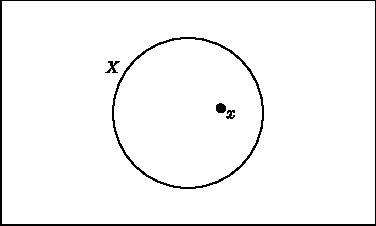
\includegraphics{../graphics/set1.pdf}
\]

\begin{definition} 
A \textbf{subset}\index{subset} $Y$ of a set $X$ is a set $Y$ such
that every element of $Y$ is also an element of $X$. We denote this
by:
\[
Y\subset X\index{set theory symbols!subset@$\subset$}
\] 
\end{definition}

If $Y$ is contained in $X$, we will sometimes loosely say that $X$ is
\textit{bigger} than $Y$.

\begin{question} 
Can you think of a set $X$ and a subset $Y$ where saying $X$ is bigger
than $Y$ is a bit misleading?
\end{question}
\QM

\begin{question} 
How is the meaning of the symbol $\in$ different from the meaning of
the symbol $\subset$?
\end{question}
\QM


\subsection{Union}


\begin{definition}\index{union}\index{u@$\cup$}\index{set theory symbols!union@$\cup$} Given two sets $X$ and $Y$, $X$ \textbf{union} $Y$ is the set of all the elements in $X$ or $Y$. We denote this by $X\cup Y$.  \fixnote{This is inclusive or.}
\end{definition}

Pictorially, we can imagine this as:

\[
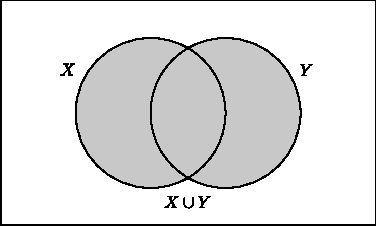
\includegraphics{../graphics/set2.pdf}
\]



\subsection{Intersection}

\begin{definition}\index{intersection}\index{set theory symbols!intersection@$\cap$} Given two sets $X$ and $Y$, 
$X$ \textbf{intersect} $Y$ is the set of all the elements that are simultaneously in $X$ and in $Y$. We denote this by $X\cap Y$. 
\end{definition}

Pictorially, we can imagine this as:
\[
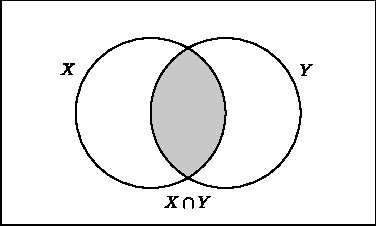
\includegraphics{../graphics/set3.pdf}
\]

\begin{question} Consider the sets $X$ and $Y$ below:
\[
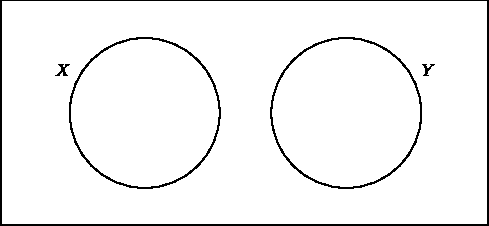
\includegraphics{../graphics/set4.pdf}
\]
What is $X\cap Y$?
\end{question}

I'll take this one: Nothing! We have a special notation for the set with no elements, it is called the \index{empty set}\textbf{empty set}. We denote the empty set by the symbol $\emptyset$.\index{set theory symbols!emptyset@$\emptyset$}  \fixnote{Include subtleties about the empty set.}




\subsection{Complement}

\begin{definition}\index{complement}\index{set theory symbols!complement@$-$} Given two sets $X$ and $Y$, 
$X$ \textbf{complement} $Y$ is the set of all the elements that are in $X$ and are not in $Y$. We denote this by $X-Y$.
\end{definition}

Pictorially, we can imagine this as:
\[
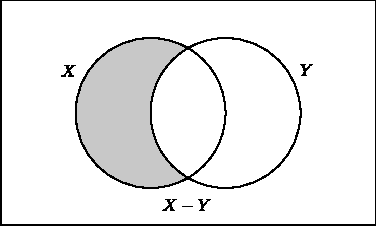
\includegraphics{../graphics/set5.pdf}
\]

\begin{question} Check out the two sets below:
\[
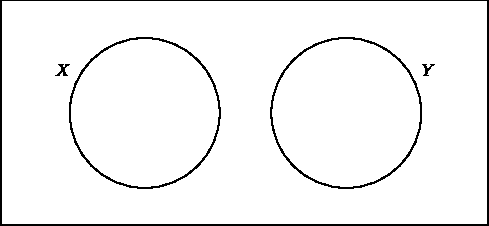
\includegraphics{../graphics/set4.pdf}
\]
What is $X-Y$? What is $Y-X$?
\end{question}
\QM


\subsection{Putting Things Together}

OK, let's try something more complex:

\begin{question} Prove that:
\[
X\cup (Y \cap Z) = (X \cup Y)\cap (X \cup Z)
\]
\end{question}

\begin{proof} 
Look at the left-hand side of the equation first. We can represent the
elements in $Y\cap Z$ with shaded region in the following diagram:
\[
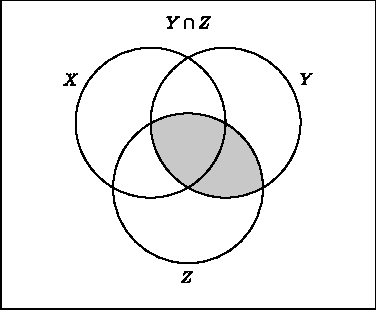
\includegraphics{../graphics/setproof.pdf}
\]
So the union of this region with $X$ is represented the shaded
region in this diagram.
\[
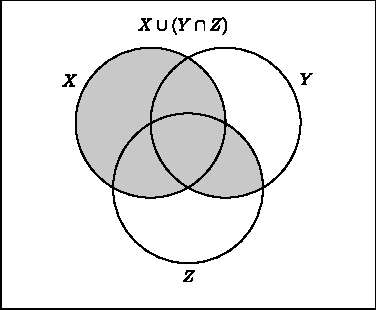
\includegraphics{../graphics/setproof1.pdf}
\]
Now, looking at the right-hand side of the equation, $X\cup Y$ is
represented by this shaded region:
\[
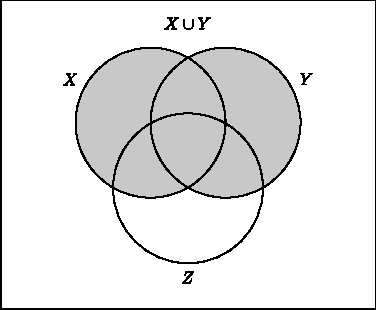
\includegraphics{../graphics/setproof2.pdf}
\]
And $X\cup Z$ is represented by this shaded region:
\[
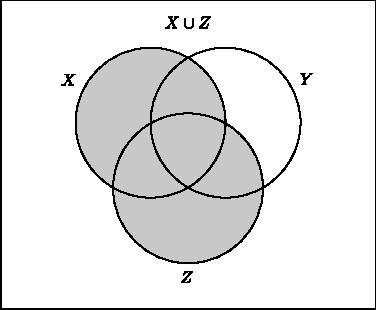
\includegraphics{../graphics/setproof3.pdf}
\]
The region shaded in both of the diagrams, which is the
intersection of $X\cup Y$ and $X\cup Z$, is represented by the shaded
region below.
\[
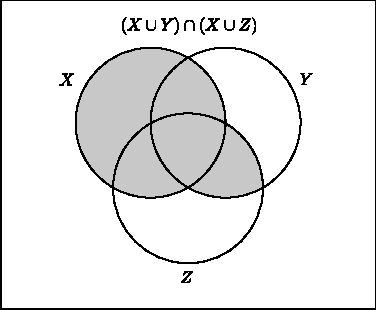
\includegraphics{../graphics/setproof4.pdf}
\]
Comparing the diagrams representing the left-hand and right-hand sides
of the equation, we see that the same regions are shaded, and so we
are done.
\end{proof}

\begin{problems}
\fixnote{Add a problem about exclusive or.}
\begin{enumerate}
\item Given two sets $X$ and $Y$, explain what is meant by $X\cup Y$.
\item Given two sets $X$ and $Y$, explain what is meant by $X\cap Y$.
\item Given two sets $X$ and $Y$, explain what is meant by $X - Y$.
\item Explain the difference between the symbols $\in$ and $\subset$.
\item If we let $X$ be the set of ``right triangles'' and we let $Y$ be the set of ``equilateral triangles'' does the picture below show the relationship between these two sets?
\[
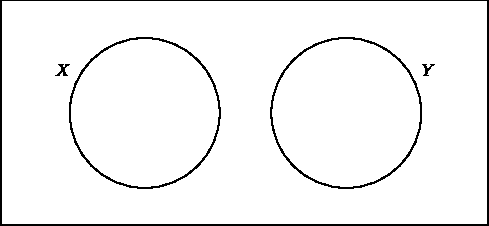
\includegraphics{../graphics/set4.pdf}
\]
Explain your reasoning.
\item If $X = \{1,2,3,4,5\}$ and $Y = \{3,4,5,6\}$ find:
\begin{enumerate}
\item $X\cup Y$
\item $X\cap Y$
\item $X-Y$
\item $Y-X$
\end{enumerate}
In each case explain your reasoning. 
\item Let $n\Z$ represent the integer multiples of $n$. So for example:
\[
3\Z = \{\dots,-12,-9,-6,-3,0,3,6,9,12,\dots\}
\]
Compute the following:
\begin{enumerate}
\item $3\Z\cap 4\Z$
\item $2\Z\cap 5\Z$
\item $3\Z\cap 6\Z$
\item $4\Z\cap 6\Z$
\item $4\Z\cap 10\Z$
\end{enumerate}
In each case explain your reasoning. 
\item Make a general rule for intersecting sets of the form $n\Z$ and
  $m\Z$. Explain why your rule works.
\item Prove that:
\[
X = (X\cap Y) \cup (X-Y)
\]
\item Prove that:
\[
X-(X-Y) = (X\cap Y)
\]
\item Prove that:
\[
X \cup (Y-X) = (X\cup Y)
\]
\item Prove that:
\[
X \cap (Y-X) = \emptyset
\]
\item Prove that:
\[
(X-Y)\cup (Y-X) = (X\cup Y)-(X\cap Y)
\]
\item Prove that:
\[
X\cup (Y \cap Z) = (X \cup Y)\cap (X \cup Z)
\]
\item Prove that:
\[
X\cap (Y \cup Z) = (X \cap Y)\cup (X \cap Z)
\]
\item Prove that:
\[
X - (Y \cap Z) = (X -Y)\cup (X - Z)
\]
\item Prove that:
\[
X - (Y \cup Z) = (X -Y)\cap (X -Z)
\]
\item If $X\cup Y = X$, what can we say about the relationship between the sets $X$ and $Y$? Explain your reasoning.
\item If $X\cup Y = Y$, what can we say about the relationship between the sets $X$ and $Y$? Explain your reasoning.
\item If $X\cap Y = X$, what can we say about the relationship between the sets $X$ and $Y$? Explain your reasoning.
\item If $X\cap Y = Y$, what can we say about the relationship between the sets $X$ and $Y$? Explain your reasoning.
\item If $X-Y =\emptyset$, what can we say about the relationship between the sets $X$ and $Y$? Explain your reasoning.
\item If $Y-X =\emptyset$, what can we say about the relationship between the sets $X$ and $Y$? Explain your reasoning.
\end{enumerate}
\end{problems}


\newpage



\section{Tessellations}

Go to the internet and look up M.C.\ Escher.\index{Escher, M.C.} He
was an artist. Look at some of his work. When you do your search be
sure to include the word ``tessellation'' OK? Back already? Very
good. Sometimes Escher worked with tessellations. What's a
tessellation? I'm glad you asked:

\begin{definition}\index{tessellation} A \textbf{tessellation} is a pattern of 
polygons fitted together to cover the entire plane without
overlapping.  
\end{definition}
While it is impossible to actually cover the entire plane with shapes,
if we give you enough of a tessellation, you should be able to continue
it's pattern indefinitely.  Here are pieces of tessellations:
\[
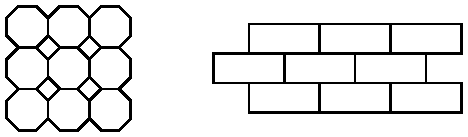
\includegraphics{../graphics/semiRegTess.pdf}
\]
On the left we have a tessellation of a square and an octagon. On the
right we have a ``brick-like'' tessellation.

\begin{definition}\index{tessellation!regular}\index{regular!tessellation}
A tessellation is called a \textbf{regular tessellation} if it is
composed of copies of a single regular polygon and these polygons meet
vertex to vertex.\index{regular!polygon}
\end{definition}


\begin{example} Here are some examples of regular tessellations:
\[
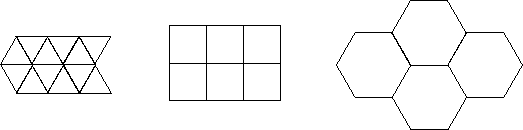
\includegraphics{../graphics/regtess.pdf}
\]
\end{example}

Johannes Kepler\index{Kepler, Johannes}, who lived from 1571--1630,
was one of the first people to study tessellations. He certainly knew
the next theorem:

\begin{theorem} There are only $3$ regular tessellations.
\end{theorem}

\begin{question} Why is the theorem above true?
\end{question}
\QM

Since one can prove that there are only three regular tessellations,
and we have shown three above, then that is all of them. On the other
hand there are lots of nonregular tessellations. Here are two
different ways to tessellate the plane with a
triangle:\index{tessellation!triangles}
\[
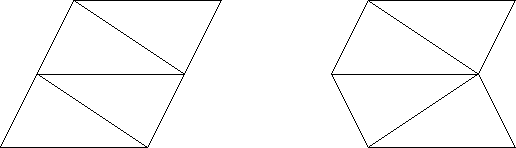
\includegraphics{../graphics/triangletess.pdf}
\]
Here is a way that you can tessellate the plane with any old
quadrilateral:
\[\index{tessellation!any quadrilateral}\index{quadrilateral!tessellation of}
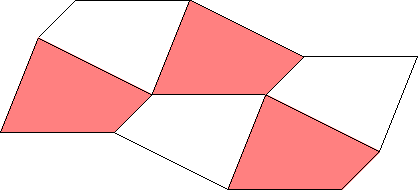
\includegraphics{../graphics/quadtess.pdf}
\]

\subsection{Tessellations and Art}

How does one make art with tessellations? To start, a little
decoration goes a long way. Check this out: Decorate two squares as
such:
\[

\includegraphics{../graphics/lightningsquares.pdf}
\]
Tessellate them randomly in the plane to get this lightning-like picture:
\[
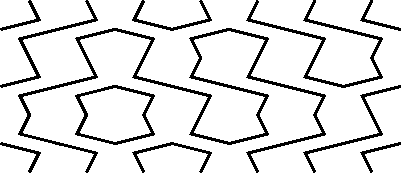
\includegraphics{../graphics/lightningtess.pdf}
\]
\begin{question} 
What sort of picture do you get if you tessellate these decorated
squares randomly in a plane?
\[
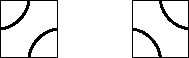
\includegraphics{../graphics/watersquares.pdf}
\]
\end{question}
\QM

Another way to go is to start with your favorite tessellation:
\[
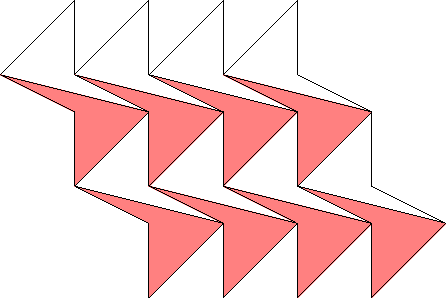
\includegraphics{../graphics/nonconvextess.pdf}
\]
Then you modify it a bunch to get something different:
\[
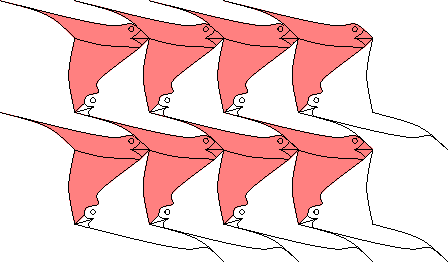
\includegraphics{../graphics/birdstess.pdf}
\]

\begin{question} What kind of art can you make with tessellations?
\end{question}
\QM


I'm not a very good artist, but I am a mathematician. So let's use a
tessellation to give a proof! Let me ask you something:

\begin{question} What is the most famous theorem in mathematics? 
\end{question}
Probably the Pythagorean Theorem comes to mind. Let's recall the statement of the Pythagorean Theorem:

\begin{theorem}[Pythagorean Theorem]\index{Pythagorean Theorem} Given a right triangle, the sum of the squares of the 
lengths of the two legs equals the square of the length of 
the hypotenuse.  Symbolically, if $a$ and $b$ represent the 
lengths of the legs and $c$ is the length of the hypotenuse, 
\[
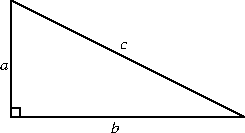
\includegraphics{../graphics/pbppyth.pdf}
\]
then 
\[
a^2 + b^2 = c^2.
\]
\end{theorem}


Let's give a proof! Check out this tessellation involving $2$ squares:
\[
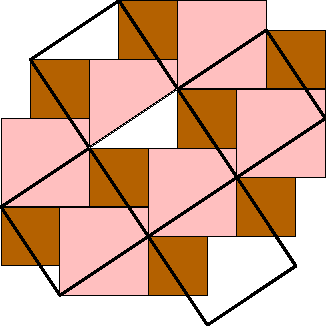
\includegraphics{../graphics/pbppyth2.pdf}
\]
\begin{question} How does the picture above ``prove'' the Pythagorean Theorem?
\end{question}
\begin{proof}[Solution]  
The white triangle is our right triangle. The area of the middle
overlaid square is $c^2$, the area of the small dark squares is $a^2$,
and the area of the medium lighter square is $b^2$. Now label all the
``parts'' of the large overlaid square:
\[
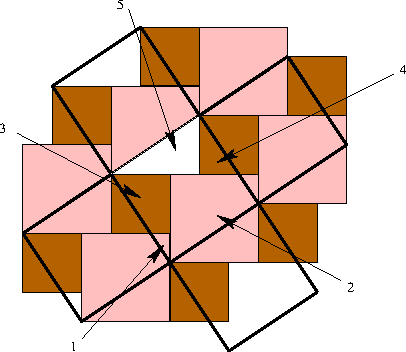
\includegraphics{../graphics/pbppyth2a.pdf}
\]
From the picture we see that
\begin{align*}
a^2 &= \{\text{3 and 4}\}\\
b^2 &= \{\text{1, 2, and 5}\}\\
c^2 &= \{\text{1, 2, 3, 4, and 5}\}
\end{align*}
Hence
\[
c^2 = a^2 + b^2
\]
Since we can always put two squares together in this pattern, this
proof will work for any right triangle.
\end{proof}

\begin{question} Can you use the above tessellation to give a dissection proof of the Pythagorean Theorem?
\end{question}
\QM



\begin{problems}

\begin{enumerate}
\item Show two different ways of tessellating the plane with a given scalene triangle. Label your picture as necessary.
\item Show how to tessellate the plane with a given quadrilateral. Label your picture.
\item Show how to tessellate the plane with a nonregular hexagon. Label your picture.
\item Give an example of a polygon with $9$ sides that tessellates the plane.
\item Give examples of polygons that tessellate and polygons that do
  not tessellate.
\item Give an example of a triangle that tessellates the plane where
  both $4$ and $8$ angles fit around each vertex.
\item True or False: Explain your conclusions.
\begin{enumerate}
\item There are exactly 5 regular tessellations.
\item Any quadrilateral tessellates the plane.
\item Any triangle will tessellate the plane.
\item If a triangle is used to tessellate the plane, then it is always
  the case that exactly $6$ angles will fit around each vertex.
\item If a polygon has more than 6 sides, then it cannot tessellate the plane.
\end{enumerate}
\item Given a regular tessellation, what is the sum of the angles
  around a given vertex?
\item Given that the regular octagon has $135$ degree angles, explain
  why you cannot give a regular tessellation of the plane with a
  regular octagon.
\item \label{tesstable} Fill in the following table:
\begin{center}
\begin{tabular}{|c || c| c| c|}\hline
 Regular & Does it      &  Measure & If it tessellates, how  \\
 $n$-gon & tessellate?  &  of an angle &  many surround each vertex?  \\
\hline\hline
$3$-gon &  &  &  \\ \hline
$4$-gon &  &  &  \\ \hline
$5$-gon &  &  &  \\ \hline
$6$-gon &  &  &  \\ \hline
$7$-gon &  &  &  \\ \hline
$8$-gon &  &  &  \\ \hline
$9$-gon &  &  &  \\ \hline
$10$-gon &  &  &  \\ \hline
\end{tabular}
\end{center}
Hint: A regular $n$-gon has interior angles of $180(n-2)/n$ degrees. 
\begin{enumerate}
\item What do the shapes that tessellate have in common?
\item Make a graph with the number of sides of an $n$-gon on the
  horizontal axis and the measure of a single angle on the vertical
  axis. Briefly describe the relationship between the number of sides
  of a regular $n$-gon and the measure of one of its angles.
\item What regular polygons \textit{could} a bee use for building
  hives? Give some reasons that bees seem to use hexagons.\index{bees}
\end{enumerate}
\item Considering that the regular $n$-gon has interior angles of
  $180(n-2)/n$ degrees, and Problem \ref{tesstable} above, prove that
  there are only 3 regular tessellations of the plane.
\item Explain how the following picture ``proves'' the Pythagorean
  Theorem.
\[
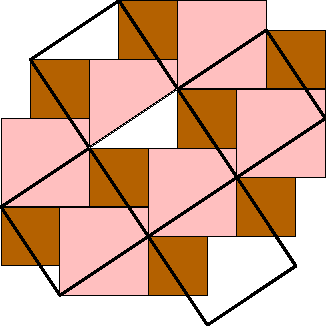
\includegraphics{../graphics/pbppyth2.pdf}
\]
\end{enumerate}
\end{problems}


\newpage



\section{Proof by Picture}
\marginnote{Most of the \textit{pictures} from this section are adapted from the wonderful source books: \cite{nelsen} and \cite{nelsen1}.}  

Pictures generally do not constitute a proof on their own. However, a
good picture can show insight and communicate concepts better than
words alone. In this section we will show you pictures giving the idea
of a proof and then ask you to supply the words to finish off the
argument. 


\subsection{Proofs Involving Right Triangles}

Let's start with something easy:

\begin{question} Explain how the following picture ``proves'' that
  the area of a right triangle is half the base times the height.
\[
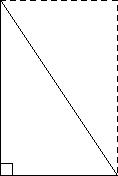
\includegraphics{../graphics/pbpAreaRight.pdf}
\]
\end{question}
\QM 

That wasn't so bad was it? Now for a game of \textit{whose-who}:

\begin{question} What is the most famous theorem in mathematics? 
\end{question}
Probably the Pythagorean Theorem comes to mind. Let's recall the statement of the Pythagorean Theorem:

\begin{theorem}[Pythagorean Theorem]\index{Pythagorean Theorem} Given a right triangle, the sum of the squares of the 
lengths of the two legs equals the square of the length of 
the hypotenuse.  Symbolically, if $a$ and $b$ represent the 
lengths of the legs and $c$ is the length of the hypotenuse, 
\[
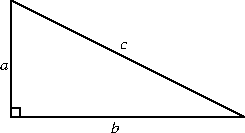
\includegraphics{../graphics/pbppyth.pdf}
\]
then 
\[
a^2 + b^2 = c^2.
\]
\end{theorem}
\begin{question} What is the converse to the Pythagorean Theorem? Is it true? How do you prove it?
\end{question}
\QM

While everyone may know the Pythagorean Theorem, not as many know how to prove it. Euclid's proof goes kind of like this: 

Consider the following picture:
\[
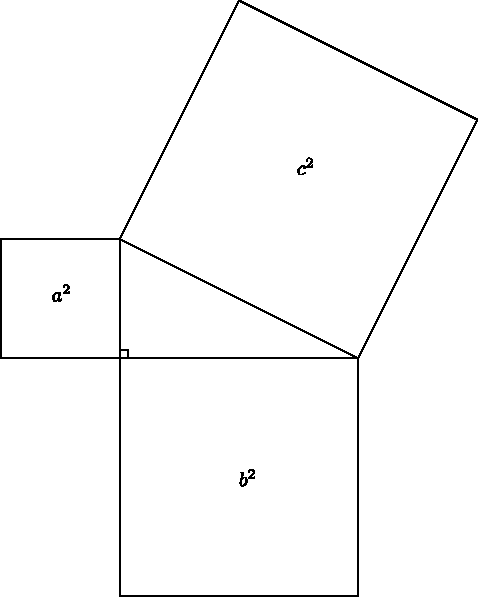
\includegraphics[scale=0.8]{../graphics/pbppythsqr.pdf}
\]
Now, cut up the squares $a^2$ and $b^2$ in such a way that they fit into $c^2$ perfectly. When you give a proof that involves cutting up the shapes and putting them back together, it is called a \textbf{dissection proof}.\index{dissection proof} The trick to ensure that this is actually a proof is in making sure
that your dissection will work no matter what right triangle you are
given. Does it sound complicated? Well it can be. 


Is there an easier proof?  Sure, look at:
\[
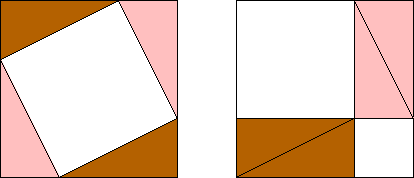
\includegraphics{../graphics/pbppyth1.pdf}
\]
\begin{question} How does the picture above ``prove'' the Pythagorean Theorem?
\end{question}


\begin{proof}[Solution] Both of the large squares above are the same size. Moreover both the unshaded regions above must have the same area. The large white square on the left has an area of $c^2$ and the two white squares on the right have a combined area of $a^2 + b^2$. Thus we see that:
\[
c^2 = a^2 + b^2
\]
\end{proof}


Now a paradox:

\begin{paradox}\index{paradox!triangle dissection} What is wrong with this picture?
\[
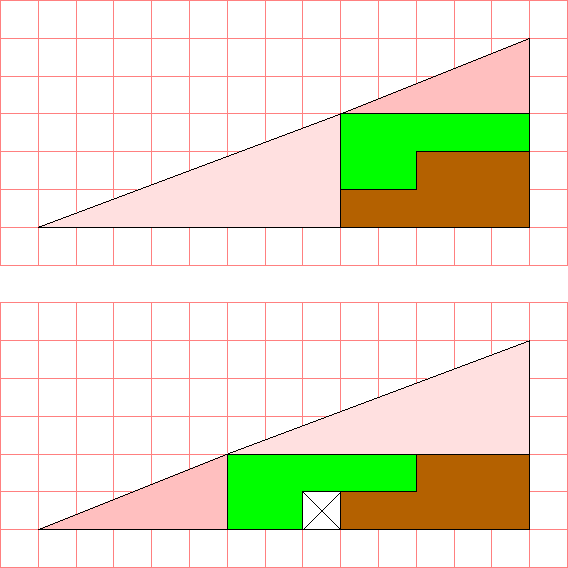
\includegraphics[scale=0.8]{../graphics/triparadox.pdf}
\]
\end{paradox}

\begin{question} 
How does this happen?   
% (See CITATION ERROR % \cite{gardner2} 
% Chapter 8, for a wonderful discussion of puzzling pictures like this one.)
\end{question}
\QM

\subsection{Proofs Involving Boxy Things}

Consider the problem of \textit{Doubling the Cube}.\index{doubling the cube} If a mathematician asks us to double a cube, he or she is asking us to double the \textbf{volume} of a given cube. One may be tempted to merely double each side, but this doesn't double the volume! 

\begin{question} Why doesn't doubling each side of the cube double the volume of the cube? 
\end{question}
\QM

Well, let's answer an easier question first. How do you double the area of a square? Does taking each side and doubling it work? 
\[
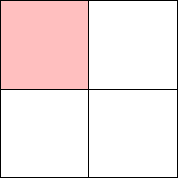
\includegraphics{../graphics/pbpsquare.pdf}
\]
No!  You now have four times the area. So you \textbf{cannot} double the area of a square merely by doubling each side.
What about for the cube? Can you double the volume of a cube merely by doubling the length of every side? Check this out:
\[
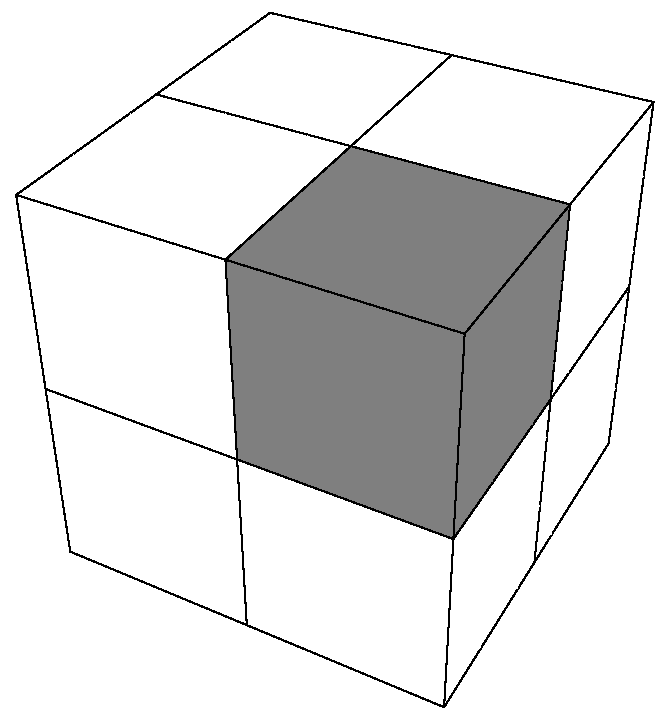
\includegraphics[scale=.4]{../graphics/119VolumeCube.pdf}
\]
Ah, so the answer is again no. If you double each side of a cube you have $8$ times the volume.

\begin{question}
What happens to the area of a square if you multiply the sides by an
arbitrary integer? What about the volume of a cube? Can you explain
what is happening here?
\end{question} 
\QM



\subsection{Proofs Involving Infinite Sums}

As is our style, we will start off with a question:

\begin{question} Can you add up an infinite number of terms and still get a 
finite number?
\end{question}


Consider $1/3$.  Actually, consider the decimal notation for $1/3$:
\[
\frac{1}{3} = .333333333333333333333333333333\dots
\]
But this is merely the sum:
\[
.3 + .03 + .003 + .0003 + .00003 + .000003 + \cdots
\]
It stays less than $1$ because the terms get so small so 
quickly.  Are there other infinite sums of this sort?  You 
bet! Check out this picture:
\[
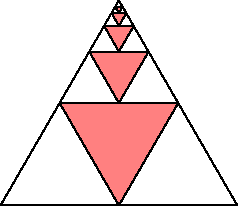
\includegraphics{../graphics/pbptriangle.pdf}
\]
\begin{question} Explain how the picture above ``proves'' that:
\[
\frac{1}{4} + \left(\frac{1}{4}\right)^2 +  \left(\frac{1}{4}\right)^3 +  \left(\frac{1}{4}\right)^4 +  \left(\frac{1}{4}\right)^5 + \cdots = \frac{1}{3}
\]
\end{question}

\begin{proof}[Solution] Let's take it in steps.  If the big triangle has area 
$1$, the area of the shaded region below is $1/4$. 
\[
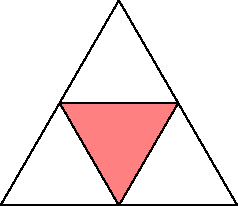
\includegraphics{../graphics/pbptriangle1.pdf}
\]
We also see that the area of the shaded region below 
\[
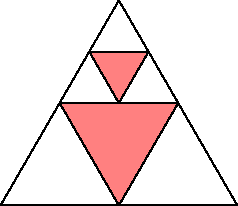
\includegraphics{../graphics/pbptriangle2.pdf}
\]
is:
\[
\frac{1}{4} + \left(\frac{1}{4}\right)^2
\]
Continuing on in this fashion we see that the area of all the shaded regions is:
\[
\frac{1}{4} + \left(\frac{1}{4}\right)^2 +  \left(\frac{1}{4}\right)^3 +  \left(\frac{1}{4}\right)^4 +  \left(\frac{1}{4}\right)^5 + \cdots
\]
But look, the unshaded triangles have twice as much area as 
the shaded triangle.  Thus the shaded triangles must have an
area of $1/3$.
\end{proof}



\subsection{Thinking Outside the Box}


A \textit{calisson}\index{calisson} is a French candy that sort of looks like two equilateral triangles stuck together. They usually come in a hexagon-shaped box. 

\begin{question} How do the calissons fit into their hexagon-shaped box?
\end{question}

If you start to put the calissons into a box, you quickly see that they can be placed in there with exactly three different orientations:
\[
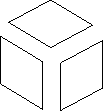
\includegraphics{../graphics/pbporicas.pdf}
\]
\begin{theorem}\label{T:cal} In any packing, the number of calissons with a given orientation is exactly one-third the total number of calissons in the box.
\end{theorem}

Look at this picture:
\[
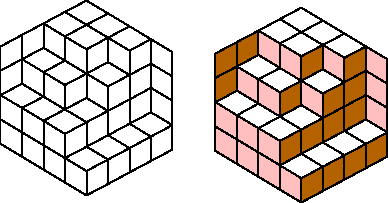
\includegraphics{../graphics/pbpcas.pdf}
\]

\begin{question} How does the picture above ``prove'' Theorem~\ref{T:cal}? Hint: Think outside the box!
\end{question}
\QM




\begin{problems}
\begin{enumerate}
\item Explain the rule
\[
\text{even} + \text{even} = \text{even}
\]
in two different ways. First give an explanation based on
pictures. Second give an explanation based on algebra. 
\item Explain the rule
\[
\text{odd} + \text{even} = \text{odd}
\]
in two different ways. First give an explanation based on
pictures. Second give an explanation based on algebra.
\item Explain the rule
\[
\text{odd} + \text{odd} = \text{even}
\]
in two different ways. First give an explanation based on
pictures. Second give an explanation based on algebra.
\item Explain the rule
\[
\text{even} \cdot \text{even} = \text{even}
\]
in two different ways. First give an explanation based on
pictures. Second give an explanation based on algebra.
\item Explain the rule
\[
\text{odd} \cdot \text{odd} = \text{odd}
\]
in two different ways. First give an explanation based on
pictures. Second give an explanation based on algebra.
\item Explain the rule
\[
\text{odd} \cdot \text{even} = \text{even}
\]
in two different ways. First give an explanation based on
pictures. Second give an explanation based on algebra.
\item\label{P:RTA} Explain how the following picture ``proves'' that
  the area of a right triangle is half the base times the height.
\[
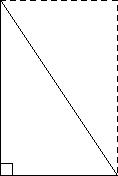
\includegraphics{../graphics/pbpAreaRight.pdf}
\]

\item Suppose you know that the area of a \textbf{right} triangle is
  half the base times the height. Explain how the following picture
  ``proves'' that the area of \textbf{every} triangle is half the base times the
  height.
\[
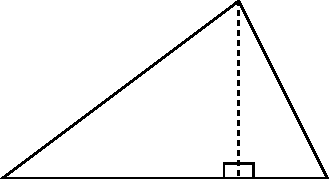
\includegraphics{../graphics/pbpDisTri.pdf}
\]
Now suppose that a student, say \textit{Geometry Giorgio} attempts to
solve a similar problem. Again knowing that the area of a right
triangle is half the base times the height, he draws the following
picture:
\[
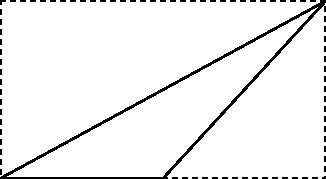
\includegraphics{../graphics/pbpDisTriGio.pdf}
\]
\textit{Geometry Giorgio} states that the diagonal line cuts the
rectangle in half, and thus the area of the triangle is half the base
times the height. Is this correct reasoning? If so, give a complete
explanation. If not, give correct reasoning based on \textit{Geometry
  Giorgio}'s picture.


\item Suppose you know that the area of a \textbf{right} triangle is
  half the base times the height. Explain how the following picture
  ``proves'' that the area of any triangle is half the base times the
  height. Note, this way of thinking is the basis for Cavalieri's
  Principle.\index{Cavalieri's Principle}
\[
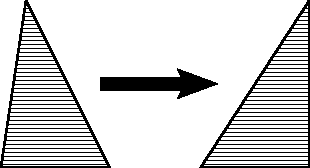
\includegraphics{../graphics/pbpShearTri.pdf}
\]
\item Explain how the following picture ``proves'' that the area of
  any parallelogram is base times height. Note, this way of thinking
  is the basis for Cavalieri's Principle.\index{Cavalieri's Principle}
\[
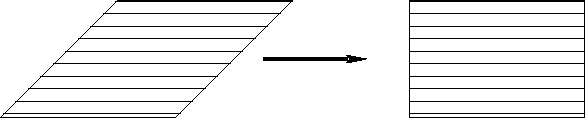
\includegraphics{../graphics/pbpShearPara.pdf}
\]

\item Explain how to use a picture to ``prove'' that a triangle of a
  given area could have an arbitrarily large perimeter.

\item Give two explanations of how the following picture ``proves''
  the Pythagorean Theorem, one using algebra and one without algebra. 
\[
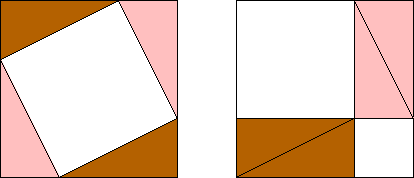
\includegraphics{../graphics/pbppyth1.pdf}
\]
\item Give two explanations of how the following picture ``proves''
  the Pythagorean Theorem, one using algebra and one without algebra. 
\[
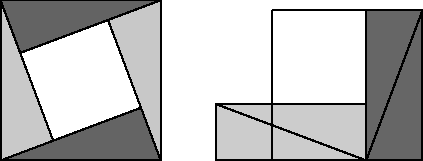
\includegraphics{../graphics/pbppyth3.pdf}
\]
\item Explain how the following picture ``proves'' the Pythagorean Theorem.
\[
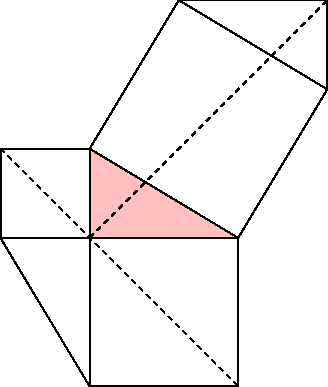
\includegraphics{../graphics/pbpdavinci.pdf}
\]
Note: This proof is due to Leonardo da Vinci.
%\item Explain how the following picture ``proves'' the Pythagorean Theorem.
%\[
%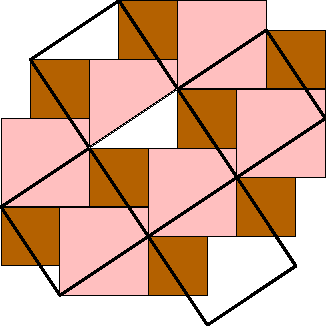
\includegraphics{../graphics/pbppyth2.pdf}
%\]
%\item Use the following tessellation to give a dissection proof of the Pythagorean Theorem.
%\[
%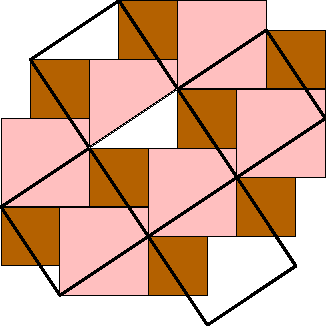
\includegraphics{../graphics/pbppyth2.pdf}
%\]
%\item Explain how the following picture ``proves'' the Pythagorean Theorem.
%\[
%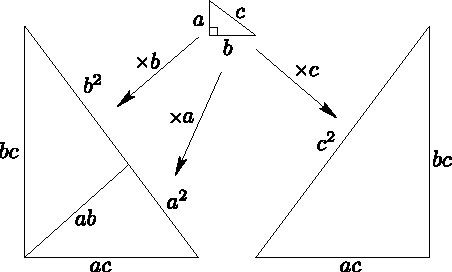
\includegraphics{../graphics/pbpdilation.pdf}
%\]
\item\label{P:pbptrap} Recall that a trapezoid is a quadrilateral with two parallel sides. Consider the following picture:
\[
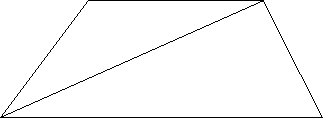
\includegraphics{../graphics/trap.pdf}
\]
How does the above picture prove that the area of a trapezoid is
\[
\mathrm{area}= \frac{h(b_1 + b_2)}{2},
\]
where $h$ is the height of the trapezoid and $b_1$, $b_2$, are the lengths of the parallel sides?
\item Explain how the following picture ``proves'' the Pythagorean Theorem.
\[
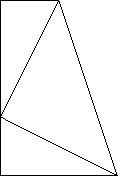
\includegraphics{../graphics/pbptrap.pdf}
\]
Note: This proof is due to James A.\ Garfield, the 20th President of the United States.
\item Look at Problem~\ref{P:pbptrap}. Can you use a similar picture
  to prove that the area of a parallelogram
\[
\includegraphics{../graphics/para.pdf}
\]
is the length of the base times the height?
\item Explain how the following picture ``proves'' that the area of a
  parallelogram is base times height.
\[
\includegraphics{../graphics/para3.pdf}
\]
Now suppose that a student, say \textit{Geometry Giorgio} attempts to
solve a similar problem. In an attempt to prove the formula for the
area of a parallelogram, \textit{Geometry Giorgio} draws the following
picture:
\[
\includegraphics{../graphics/paragiorgio.pdf}
\]
At this point \textit{Geometry Giorgio} says that he has proved the
formula for area of a parallelogram. What do you think of his picture?
Give a complete argument based on his picture.

\item Which of the above ``proofs'' for the formula for the area of a
  parallelogram is your favorite? Explain why.

\item Explain how the following picture ``proves'' that the area of a
  quadrilateral is equal to half of the area of the parallelogram
  whose sides are parallel to and equal in length to the diagonals of
  the original quadrilateral.
\[
\includegraphics[scale=.7]{../graphics/pbpquadarea.pdf}
\]

\item Explain how the following picture ``proves'' that if a
  quadrilateral has two opposite angles that are equal, then the
  bisectors of the other two angles are parallel or on top of each
  other.
\[
\includegraphics[scale=.7]{../graphics/119hw5_2.pdf}
\]



\break

\item\label{P:Tparadox1} Why might someone find the following picture
  disturbing? How would you assure them that actually everything is
  good and well in the geometrical world?
\[
\includegraphics[scale=.8]{../graphics/triparadox.pdf}
\]



\item\label{P:Tparadox2} Why might someone find the following picture
  disturbing? How would you assure them that actually everything is
  good and well in the geometrical world?
\[
\includegraphics[scale=.8]{../graphics/triparadox2.pdf}
\]


\item How could you explain to someone that doubling the lengths of each side of a cube does not double the volume of the cube?

\item\label{P:sq1}  Explain how the following picture ``proves'' that:
\[
\frac{1}{2} + \left(\frac{1}{2}\right)^2 +  \left(\frac{1}{2}\right)^3 +  \left(\frac{1}{2}\right)^4 +  \left(\frac{1}{2}\right)^5 + \cdots = 1
\]
\[
\includegraphics{../graphics/pbpsqgeo.pdf}
\]
\item\label{P:sq2}  Explain how the following picture ``proves'' that if $0 < r < 1$:
\[
r + r(1-r) + r(1-r)^2 + r(1-r)^3 + \cdots = 1
\]
\[
\includegraphics{../graphics/pbpgengeo.pdf}
\]
\item\label{P:tri1} Explain how the following picture ``proves'' that:
\[
\frac{1}{4} + \left(\frac{1}{4}\right)^2 +  \left(\frac{1}{4}\right)^3 +  \left(\frac{1}{4}\right)^4 +  \left(\frac{1}{4}\right)^5 + \cdots = \frac{1}{3}
\]
\[
\includegraphics{../graphics/pbptriangle.pdf}
\]
\item Considering Problem~\ref{P:sq1}, Problem~\ref{P:sq2}, and
  Problem~\ref{P:tri1} can you give a new picture ``proving'' that: 
\[
\frac{1}{4} + \left(\frac{1}{4}\right)^2 +  \left(\frac{1}{4}\right)^3 +  \left(\frac{1}{4}\right)^4 +  \left(\frac{1}{4}\right)^5 + \cdots = \frac{1}{3}
\]
Carefully explain the connection between your picture and the
mathematical expression above.

\item Explain how the following picture ``proves'' that  in any packing, the number of calissons with a given orientation is exactly one-third the total number of calissons in the box.
\[
\includegraphics{../graphics/pbpcas.pdf}
\]
\end{enumerate}
\end{problems}


\chapter{Toward Congruence and Similarity}  

%Key pieces
%\begin{itemize}
%\item Transformations and symmetries
%\item Congruence via isometries
%\item Parity of isometries
%\item 1166 parallel postulate
%\item Similarity via dilations
%\end{itemize}

\section{Transformations, Symmetry, and Congruence}
In school mathematics, transformations and symmetry have typically been small niche topics, separate from each other, separate from most of the rest of school mathematics, and receiving little curricular attention.  Congruence, on the other hand, is a more prominent idea that begins informally in the elementary grades as ``same shape, same size'' and culminates in high school with axioms, theorems, and proofs.  

In this section, we demonstrate how transformations can undergird both symmetry and congruence, thereby strengthening all three topics and also establishing groundwork for an analogous approach to similarity.  

\subsection{Transformations}
Informally, a transformation of the plane is a ``motion,'' such as a rotation or a stretch of the plane.  More formally, a transformation is a function that takes points in the plane as inputs and gives points as outputs.\standardhs{G-CO.2}  In school mathematics, we consider only transformations that take lines to lines, so that key geometric features are ``preserved.''  For example a triangle remains a triangle when it is rotated and even when it is stretched.  

Transformations are often specified using a coordinate system, but coordinates are not necessary.  For now, we will explore transformations without a coordinate system.  Later, we will use coordinates, along with matrices and vectors, to describe transformations.  

\begin{definition}
Transformations that preserve distances and angles are called \emph{isometries}, and the most important of these are \emph{basic rigid motions}: translations, rotations, and reflections.  
\end{definition}

\begin{question}
Is a transformation that stretches the plane an isometry?  Explain.  
\end{question}
\QM

Through exploration with transparencies, tracing paper, software,\standardhs{G-CO.2} it is not hard to see that the basic rigid motions have important properties.\standard{8.G.1} \standard{8.G.1a} \standard{8.G.1b} \standard{8.G.1c}  Based on such explorations, we write careful definitions of translation, reflection, rotation, by considering what is required to specify each transformation.\standardhs{G-CO.4}

\begin{definition}
The \emph{identity transformation}, sometimes called the ``do nothing'' transformation, doesn't move the plane at all.  As a function, the identity transformation takes a point to itself: The output is identical to the input.
\end{definition}

\begin{question}
Is the identity transformation a translation, rotation, or reflection?  Explain.  
\end{question}
\QM 

\subsection{Symmetry}
A \emph{symmetry} of a figure is a transformation that takes the figure onto itself, so that the figure is ``preserved'' by the transformation.  In everyday language, we sometimes say a figure is ``symmetrical,'' but mathematically we can be more precise by specifying the symmetry transformation(s) of the figure.\standardhs{G-CO.3}  

\begin{question}
What are the symmetries of a rectangle?  Be sure to specify the transformations.  
\end{question}
\QM

\subsection{Congruence}
Congruence is often defined using angles and side lengths.  But such a definition cannot apply to figures that are not polygons.  A more inclusive definition is as follows:  

\begin{definition}
Two figures (in the plane) are said to be \emph{congruent} to one another if there is a sequence of basic rigid motions that takes one figure onto the other.  
\end{definition}

The idea behind this definition is sometimes called the \emph{principle of superposition}, which states that congruent figures can be placed exactly on top of one another.  The above definition is more precise than superposition because it calls for an explicit sequence of basic rigid motions (e.g., translations, rotations, and reflections) rather than merely ``movement'' of one figure onto the other.  

\begin{question}
When we say that two polygons are congruent, why is the order of labeling the vertices important?  For example, if we know $\tri ABC \simeq \tri XYZ$, does it follow that $\tri ABC \simeq \tri YXZ$?  Explain.  (Hint:  Which angle of $\tri XYZ$ corresponds to $\angle A$?  Which side of $\tri ABC$ corresponds to $\overline{XZ}$?)
\end{question}
\QM

The above definition of congruence helps us in two directions.\standard{8.G.2}  First, if we have a sequence of basic rigid motions that takes one figure onto another, then we know the two figures are congruent.  Furthermore, the sequence of basic rigid motions sets up the correspondences between various parts of the figures.  Conversely, if two figures are congruent, then we know it is possible to find a sequence of basic rigid motions that takes one figure onto the other.  And the sequence of basic rigid motions often takes advantage of corresponding parts that are already known to be congruent. 

For triangles, we still have the familiar congruence criteria, such as side-side-side (SSS), side-angle-side (SAS), and angle-side-angle (ASA).  The key idea is that although triangles have six measures of sides and angles, most of the time (but not always) just three of these measures are sufficient to determine the triangle uniquely.  Students can develop intuition about these criteria by drawing triangles from given conditions.\standard{7.G.2}  The next step is to show, first, that the above definition fits with traditional notions of triangle congruence\standardhs{G-CO.7}, and, second, to prove that the triangle congruence criteria follow from the properties of the basic rigid motions.\standardhs{G-CO.8}

%To connect this definition of congruence with familiar notions of congruence, there are three parts:  
%
%Show that the if two triangles are congruent via rigid motions, then they are congruent in the familiar 
%sense of congrent angles and sides.  


\begin{problems}
\begin{enumerate}

\item What is required to specify a translation?  
\item What is required to specify a rotation? 
\item What is required to specify a reflection?  

Sometimes a sequence of transformations can be described as a single translation, rotation, or reflection.  

\item What kind of transformation is a translation followed by a translation?  Explain.  Be sure to consider any special cases.  
\item What kind of transformation is a rotation followed by a rotation?  Explain.  Be sure to consider any special cases.   
\item What kind of transformation is a reflection followed by another reflection?  Explain.  Be sure to consider any special cases.  

\item Will the letter P look like a P after a reflection?  What about after a sequence of two reflections?  What about after a sequence of 73 or 124 reflections?  Explain your reasoning.  

\item How will your answer to the previous problem change if you use a capital D?  Explain.  

\item Given a figure and its image after a translation, how do find the direction and distance of the translation?    How many points and images do you need?  
\item Given a figure and its image after a reflection, how do you find the line of reflection?  How many points and images do you need?  
\item Given a figure and its image after a rotation, how do you find the center and the angle of the rotation?  How many points and images do you need?  

\item Categorize the capital letters of the alphabet by their symmetries.  

\item Write the words COKE and PEPSI in capital letters so that they read vertically.  Use a mirror to look at a reflection of the words.  What is different about the reflections of the two words?  Explain.  

\item Describe all of the symmetries of the following figures: 
\begin{enumerate}
\item An equilateral triangle
\item An isosceles triangle that is not equilateral
\item A square
\item A rectangle that is not a square
\item A rhombus that is not a square
\item A (non-special) parallelogram
\item A regular $n-$gon
\end{enumerate}

\item What are the symmetries of a circle? 

\item How can you use the symmetries of a circle to determine whether a figure is indeed a circle?  

\item What are the symmetries of a line?  
\begin{enumerate}
\item Describe all translation symmetries.  
\item Describe all rotation symmetries.
\item Describe two types of reflection symmetries.
\item Given a line, describe a rotation symmetry and a reflection symmetry that have the same effect on a line.  How do the corresponding transformations differ in what they do to the surrounding space?  
\end{enumerate}

\item How can you use the symmetries of a line to determine whether a figure is indeed a line? 

\item Find some tessellations.  For each tessellation, describe all of its symmetries.  

\end{enumerate}

\end{problems}

\newpage 

\section{Euclidean and non-Euclidean Geometries}
The geometry of school mathematics is called \emph{Euclidean Geometry} for it is the geometry organized and detailed by Euclid more than 2,000 years ago.  To better understand the assumptions that underlie Euclidean geometry and the results that follow, it helps to be aware of non-Euclidean geometries.  Perhaps the most accessible of these is spherical geometry, because we can make use of basketballs that we can hold in our hands, and we can take advantage of our experience traveling on our (approximately spherical) Earth, modeled by a globe.  

To think about spherical geometry, it helps to imagine a bug crawling on the surface of a sphere.  From the bug's perspective, the surface of the sphere is very much the same as the surface of a Euclidean plane.  Both surfaces are two-dimensional in the sense that the bug has two degrees of freedom:  forward/backward and left/right.  Any other movement can be expressed as a combination of these.  (We are assuming the bug must stay \emph{on the surface}:  It can neither fly away from nor burrow underneath the surface.)  Whereas the surface of a Euclidean plane is infinite and flat, the surface of a sphere is finite and curved.  But if the sphere is reasonably large (compared to the bug), then even a very smart bug might have trouble determining whether she or he was walking on a sphere or on a flat plane.

Points in spherical geometry are taken to be points on the surface of the sphere.  But ``lines'' present more of a challenge:  We want lines to be ``straight'', but any path on the surface of a sphere curves with the surface.  Suppose the bug travels forward along a path that is as straight as possible, being very careful to veer neither right nor left.  Alternatively, because lines should determine ``shortest paths'' between two points, stretch a rubber band between two points on a basketball or on a globe to find the shortest path.  (Try this!)  In both cases, you will find that best answer is that a ``line'' in spherical geometry is a \emph{great circle}, which is to say a circle that is as big as possible on the sphere.  From a three-dimensional perspective, the center of a great circle is the same as the center of the sphere.  
\begin{question}
Are longitude lines on the earth ``lines'' in spherical geometry?  What about latitude lines?  Explain your reasoning.  
\end{question}
$$\includegraphics[scale=0.7]{../graphics/spherical1}$$
\QM

% Intrinsic vs. extrinsic curvature.  geodesics.  

In non-Euclidean geometries, many familiar results no longer hold.  In spherical geometry, for example, there are no parallel lines because any two lines intersect in two points, and the sum of the angles in a triangle is greater than $180^\circ$.  In hyperbolic geometry, in contrast, parallel lines are not a fixed distance apart, the sum of the angles in a triangle is less than $180^\circ$.  
$$\includegraphics[scale=0.7]{../graphics/spherical2}$$

The following statements characterize three different types of geometries:  
\begin{itemize}
\item Euclidean geometry: Given a line and a point not on the line, there is \emph{exactly one line} parallel to the given line.

\item Spherical geometry:  Given a line and a point not on the line, there are \emph{no lines} through the point parallel to the given line. 

\item Hyperbolic geometry:  Given a line and a point not on the line, there is \emph{more than one line} parallel to the given line. 
\end{itemize}

% Each of these geometries requires other postulates, of course.  Here we are merely highlighting a crucial distinction among them.  


In this course, we explore neither spherical nor hyperbolic geometry in detail, but keep these contrasting ideas in mind as we continue to dig into Euclidean geometry.  

\begin{problems}

\begin{enumerate}

\item From the above statements about angle sums in triangles, what can you conclude about angle sums in quadrilaterals  in spherical and hyperbolic geometries?

\item In Euclidean geometry, a rectangle is a quadrilateral with four right angles. 
\begin{enumerate}
\item What can you conclude about rectangles in spherical and hyperbolic geometries?  Explain.  
\item What does this imply about the usefulness of familiar (Euclidean) area formulas in these other geometries?  Explain your reasoning. 
\end{enumerate} 

\item A bear goes traveling.  She walks due south for one mile, turns left $90^\circ$, and walks due east for one mile.  She again turns left $90^\circ$, and then walks due north for one mile, ending in the place where she started.  What color is the bear?  Explain your reasoning.  

\item When walking on a sphere, how could a bug check whether she or he was traveling straight.  

\item In the Euclidean plane, any two distinct points determine a unique line.  Is that true in spherical geometry?  

\item Can the Euclidean definition of a circle make sense on a sphere?  Be sure that the center of the circle is a point on the sphere.  How would you measure the radius of the circle?  

% finding routes of planes or ships on the globe.  Get back to latitude lines. 

% rotations, reflections, and translations on a sphere? 

% Is radius perpendicular to tangent to circle?  

% poles of a great circle  

% perhaps compare area and circumference of the spherical and Euclidean circle.  

%  Problems about symmetries of a line on the sphere.  Use it to argue that great circles are straight.  
% Wrapping a ribbon on a sphere.    
% driving a car with fixed wheels (distance traveled). 


% Betweenness collapses. 
% Two points do not always determine a unique line.  
% antipodal points lie on opposite ends of a diameter
% lines are finite in extent
% perpendicular from a point to a line is not necessarily unique.
% exterior angle theorem 


\end{enumerate}

\end{problems}

\newpage 

\section{Assumptions in Mathematics}
Every area of mathematics is based on a set of assumptions, sometimes called axioms or postulates,\margincomment{In classical mathematics, ``axioms'' were self-evident statements that were common to many areas of science (including mathematics), whereas ``postulates'' were common-sense facts drawn from experience in specific areas, such as geometry.  In modern mathematics, this distinction is no longer seen as significant, and most assumptions are merely called axioms.  In deference to Euclid's \emph{Elements}, the word postulate is used almost exclusively to discuss key assumptions in geometry, as you will see below.}
which are merely statements that are accepted without proof.  They serve as the foundation of the theory being developed, and all other facts are proven beginning with these assumptions.  This approach is called the \emph{axiomatic method}.  

\dots Or at least that's how mathematics is imagined to work.  In practice, because mathematics is so vast and interconnected, most mathematical reasoning and problem solving starts ``in the middle'' from a collection of accepted facts, with little worry about which statements were taken as assumptions and which were proven as theorems.  

And there are choices.  For example, to build Euclidean geometry, we may choose any one of the following statements as an axiom and then prove the other two as theorems:   
\begin{itemize}\parsep0pt\parskip0pt
\item Given a line and a point not on the line, there is \emph{exactly one line} parallel to the given line.
\item If parallel lines are cut by a transversal, then corresponding angles are congruent.
\item The sum of the interior angles of a triangle is $180^\circ$.
\end{itemize}

In these notes, we take the first statement as an axiom, and we prove the other two statements.  

% Incorporate meanings of fractions, and the fundamental assumption of school mathematics.  

\begin{question}
In school mathematics we can ``explain'' the properties of whole or rational numbers by appealing to models and to meanings of the arithmetic operations.  But in advanced mathematics courses, the real numbers are usually specified via axioms, some of the axioms have names.  What are the names of the following axioms:  
\begin{enumerate}
\item $a + b = b + a$  
\item $a(bc) = (ab)c$
\item $a(b+c) = ab + ac$
\item If $a = b$ and $b = c$ then $a = c$ 
\end{enumerate}
\end{question}
\QM

Chances are you used the word ``property'' or ``law'' rather than ``axiom'' in your response.  Some of the properties have important names, such as the \emph{distributive property of multiplication over addition}.  The last of these is called the transitive property of equality.  But in school mathematics, it is neither necessary to instructive to insist that every such property have a shared name.  

% Much of school mathematics proceeds along the same lines:  axioms, assumptions, and postulates are rarely explicit; 
% and outside of the high school geometry course, about the only fact that is called a theorem is that of Pythagoras. 

\subsection{Assumptions for School Geometry}
We propose the following set of assumptions\margincomment{In addition to these geometric assumptions, we of course assume the properties of the algebra of real numbers.} for school geometry:  
{\small
\begin{itemize}
\item[(A1)] Through two distinct points passes a unique line.
\item[(A2)] Given a line and a point not on the line, there is exactly one line passing through the point which is parallel to the given line (Parallel postulate).
\item[(A3)] The points on a line can be placed in one-to-one correspondence with the real numbers so that differences measure distances (Ruler postulate).  
\item[(A4)] The rays with a common endpoint can be numbered so that differences measure angles and so that straight angles measure $180^\circ$ (Protactor postulate). 
\item[(A5)] Every basic rigid motion (rotation, reflection, or translation) has the following properties:
\begin{enumerate}[(i)]\parskip0pt
\item It maps a line to a line, a ray to a ray, and a segment to a segment.
\item It preserves distance and angle measure.
\end{enumerate}
\item [(A6)] Areas of geometric figures have the following properties: 
\begin{enumerate}[(i)]%\parskip0pt\parsep0pt
\item Congruent figures enclose equal areas.
\item Area is additive, i.e., the area of the union of two regions that overlap only at their boundaries is the sum of their areas. 
%\item Area is measured by tiling a region with a two-dimensional unit (such as a square) and parts of the unit, without gaps or overlaps. 
\item A rectangle with side-lengths $a$ and $b$ has area $ab$, where $a$ and $b$ can be any non-negative real numbers.
\end{enumerate}

\end{itemize}
}

\bigskip

These assumptions can be remembered easily in the following chunks:  
\begin{itemize}
\itemsep0em
\item (A1) and (A2):  Points, lines, and parallel lines behave as they should. 
\item (A3) and (A4):  Distance and angle measure behave as they should. 
\item (A5):  Basic rigid motions behave as they should.
\item (A6):  Area behaves as it should.  
\end{itemize}

\begin{question}
Given two distinct lines, if they have no points in common, they are said to be parallel.  Most of the time, of course, they will have exactly one point in common.  Can the two lines have more than one point in common?  Use the above axioms to explain your reasoning.  
\end{question}

%Lemma 2. If three lines L1, L2, and L3 have the property that L1 || L2 and L2 || L3,
%then L1 || L3.

The ruler postulate gives us a definition of betweenness, which allows to to define line segment and ray.    

\begin{definition}
If points $A$, $X$, and $B$ are on a line $l$, we say that $X$ is \emph{between} $A$ and $B$ if $AX + XB = AB$.
\end{definition}

\begin{question}
Use the concept of betweenness to define line segment $\overline{AB}$.  Now use the concept of betweenness to define ray $\overrightarrow{AB}$. 
\end{question}

\begin{question}
Use the protractor postulate to provide a definition of adjacent angles, analogous to betweenness for distances.  
\end{question}

\begin{question}
Prove:  Let $l$ be a line and $O$ be a point on $l$. Let $R$ be the $180^\circ$
rotation around $O$. Then $R$ maps $l$ to to itself.  (Hint:  Pick points $P$ and $Q$ on $l$ so that $O$ is between them, and consider the straight angle $\angle POQ$.)
\end{question}

\begin{theorem}
Let $l$ be a line and $O$ be a point \emph{not} lying on $l$. Let $R$ be the $180^\circ$
rotation around $O$. Then $R$ maps $l$ to a line parallel to itself. 
\end{theorem}

Note:  The following proof uses function notation to describe the images under the rotation $R$.  Thus $R(l)$ is the image of line $l$, and $R(Q)$ is the image of point $Q$.  

\begin{proof}
Suppose $R(l)$ is not parallel to $l$.  Then $R(l)$ and $l$ have a point $Q$ in common.  Because $Q$ is on $R(l)$, there is a point $P$ on $l$, 
so that $R(P) = Q$. Because $R$ is a $180^\circ$ rotation around $O$, the three points $P$, $Q$, and $O$ lie in a line $m$. But
$Q$ is by assumption also a point in $l$, so $l$ and $m$  have two distinct points in common: $P$ and $Q$. 
But $l$ and $R(l)$ are distinct because $O$ is on $m$ but not on $l$. We have a contradiction, and thus $R(l)$ must be parallel to $l$.  
\end{proof}

%Lemma 1 (page 81) and Theorem 1 is proved.
%
%Corollary. Given a line L and point P not on L, there is a line parallel to L and
%passing through P.
%
%Pick Q on L.  Let O be the midpoint of PQ, and use Theorem 1.  
%
%Theorem 2. Two lines perpendicular to the same line are either identical or parallel


\begin{problems}
\begin{enumerate}
\item Use adjacent angles to prove that vertical angles are equal.    
\item Now use rotations to prove that vertical angles are equal.

\item Prove that alternate interior angles and corresponding angles of a transversal with respect to a pair of parallel lines are equal.
\item Prove that the sum of the interior angles of a triangle is $180^\circ$.
\item Prove: If a pair of alternate interior angles or a pair of corresponding angles of a transversal with respect to two lines are equal, then the lines are parallel.
\end{enumerate}
\end{problems}


\section{Dilations, Scaling, and Similarity}
In a previous section, we saw how transformations can be used as a foundation for describing congruence and explaining the triangle congruence criteria.  In this section, we show how transformations can be used to describe similarity.  Because the basic rigid motions all preserve distances, we need a new kind of transformation:  a dilation. 

\begin{definition}
Given a point $O$ and a positive number $r$, a \emph{dilation} about $O$ by scale factor $r$, is a mapping that takes a point $P$ to a point $P'$ so that $OP' = r\cdot OP$.  
\end{definition}

With this definition, rubber bands are natural tools for exploring dilations.  By tying together two rubber bands 
Through explorations with rubber bands and with geometry software, we observe that a dilation has the following properties:\standardhs{G-SRT.1}%\standardhs{G-SRT.1a}\standardhs{G-SRT.1b}  

\begin{enumerate}[(i)]\parskip0pt\parsep0pt
\item It maps lines to lines, rays to rays, and segments to segments.
\item It changes distance by a factor of $r$, where $r$ is the scale factor of the dilation.
\item It maps every line passing through the center of dilation to itself, and it maps every line not passing through the center of the dilation to a parallel line.  
\item It preserves angle measure.
\end{enumerate}

We could assume these properties, just as we have assumed the properties of the basic rigid motions.  It is possible to use our assumptions about area to prove some of these properties.  These are the Side-Splitter Theorems.\standard{8.G.4}  


\begin{definition}
A geometric figure is \emph{similar} to another if the second can be obtained from the first by a sequence of rotations, reflections, translations, and dilations.  
\end{definition}

If the objects are similar, try to find a single dilation that demonstrates the similarity.   If you cannot find such a dilation, explain how you know you cannot.  


\section{Length, Area, and Volume Under Scaling}

\fixnote{To be written.}  

\fixnote{Include problems on making scale drawings and on using scale drawings to solve problems about length and area.}

\fixnote{Also need to write a section for parametric equations, coordinates, functions.}

%
 \chapter{CCSS Grade 8 to HS Geometry}  

\section{Grade 8}
In school mathematics, transformations and symmetry have typically been small niche topics, separate from each other, separate from most of the rest of school mathematics, and receiving little curricular attention.  Congruence, on the other hand, is a more prominent idea that begins informally in the elementary grades as ``same shape, same size'' and culminates in high school with axioms, theorems, and proofs.  

Understand congruence and similarity using physical models, transparencies, or geometry software.
\standard{8.G.1} \standard{8.G.1a} \standard{8.G.1b} \standard{8.G.1c}
\standard{8.G.2}
\standard{8.G.3}
\standard{8.G.4}
\standard{8.G.5}

Understand and apply the Pythagorean Theorem.
\standard{8.G.6}
\standard{8.G.7}
\standard{8.G.8}

Solve real-world and mathematical problems involving volume of
cylinders, cones, and spheres.
\standard{8.G.9}

\section{High School Geometry}
In school mathematics, transformations and symmetry have typically been small niche topics, separate from each other, separate from most of the rest of school mathematics, and receiving little curricular attention.  Congruence, on the other hand, is a more prominent idea that begins informally in the elementary grades as ``same shape, same size'' and culminates in high school with axioms, theorems, and proofs.  

Experiment with transformations in the plane
\standardhs{G-CO.1}
\standardhs{G-CO.2}
\standardhs{G-CO.3}
\standardhs{G-CO.4}
\standardhs{G-CO.5}

Understand congruence in terms of rigid motions
\standardhs{G-CO.6}
\standardhs{G-CO.7}
\standardhs{G-CO.8}

Prove geometric theorems
\standardhs{G-CO.9}
\standardhs{G-CO.10}
\standardhs{G-CO.11}

Make geometric constructions
\standardhs{G-CO.12}
\standardhs{G-CO.13}

Understand similarity in terms of similarity transformations
\standardhs{G-SRT.1}\standardhs{G-SRT.1a}\standardhs{G-SRT.1b}
\standardhs{G-SRT.2}
\standardhs{G-SRT.3}

Prove theorems involving similarity
\standardhs{G-SRT.4}
\standardhs{G-SRT.5}

Define trigonometric ratios and solve problems involving right
triangles
\standardhs{G-SRT.6}
\standardhs{G-SRT.7}
\standardhs{G-SRT.8}

Apply trigonometry to general triangles
\standardhs{G-SRT.9}
\standardhs{G-SRT.10}
\standardhs{G-SRT.11}


\appendix

\renewcommand{\theenumi}{$(\mathrm{\alph{enumi}})$}
\renewcommand{\labelenumi}{\theenumi}
\chapter{Supplemental Activities}

%\setcounter{page}{1}
%\setcounter{section}{43}


\newpage

\section{Measuring Area}

\begin{prob}
Three congruent triangles are shown below.   
\begin{enumerate}
\item For each triangle, choose a base and use a ruler to draw carefully the corresponding height to that base.  (Choose bases of different lengths.)  Remember:  A \emph{height} is a measured on a line that is perpendicular to a base and containing the opposite vertex. 
\item Measure the heights and bases accurately, and compute the area of each triangle.  
\item What do your results demonstrate about the formula for the area of a triangle?  
\end{enumerate}

\begin{fullwidth}
\includegraphics{../graphics/triangle.pdf}
\includegraphics{../graphics/triangle.pdf}
\includegraphics{../graphics/triangle.pdf}
\end{fullwidth}

\end{prob}

\newpage

\section{Triangle Investigation}

\begin{prob}
Use informal reasoning to draw triangles based on the conditions given below.  You may use ruler, protractor, and/or compass if you wish, but your solutions should come from reflection and reasoning on you work.  In each part, determine whether the information provided determines a unique $\triangle ABC$, more than one triangle, or no triangle.\standard{7.G.2}   Note:  To check to see if two triangles are different, attempt to lay one directly on top of the other.  

\begin{enumerate}

\item $AB = 4$ and $BC = 5$
\item $m\angle CAB = 25^\circ$, $m\angle ABC = 75^\circ$, $m\angle BCA = 80^\circ$
\item $m\angle CAB = 25^\circ$, $m\angle ABC = 65^\circ$, $m\angle BCA = 80^\circ$
\item $AB = 5$, $m\angle BAC = 30^\circ$, $m\angle ABC = 45^\circ$
\item $AB = 5$, $BC = 4$, $m\angle ABC = 60^\circ$
\item $BC = 7$, $CA = 8$, $AB = 9$
\item $BC = 4$, $CA = 8$, $AB = 3$
\item $m\angle ABC = 45^\circ$, $BC = 8$, $CA = 12$
\item $m\angle ABC = 30^\circ$, $BC = 10$, $CA = 7$
\item $m\angle ABC = 60^\circ$, $BC = 10$, $CA = 3$

\end{enumerate}

\end{prob}

\newpage

\section{Tilted Square}

\begin{prob}
In the diagram below, the dots are 1 centimeter apart, both vertically and horizontally.  The vertices of the square all lie exactly on such dots. Find the area of the square, \emph{without computing the length of the side of the square}.  Explain your method.  

\includegraphics{../graphics/tiltedSquare}

\end{prob}

\newpage

\section{Pythagorean Theorem}

\begin{prob}
Give two explanations of how the following picture ``proves''
  the Pythagorean Theorem, one using algebra and one without algebra.\standard{8.G.6} 
\[
\includegraphics[scale=1.3]{../graphics/pbppyth1.pdf}
\]

\end{prob}

\vfill

\begin{prob}
State the converse of the Pythagorean Theorem and prove it.  
\end{prob}
\vfill

\newpage

\section{Trapezoid Area}

\begin{prob}
In this activity, we explore several ways of justifying the formula for the area of a trapezoid, as labeled below. 
\[
\includegraphics[scale=0.6]{../graphics/trapezoid1.pdf}
\]
Complete the table on the following page so that in each row the explanation, the figure, and the area formula together describe a way of computing the area.  For comparison purposes, each illustration should include a trapezoid congruent to the trapezoid above.   

All of the area formulas will, of course, be equivalent to one another as expressions.  But each way of expressing the area will make the most sense with figure and the explanation from the same row.  

\newpage

\newlength{\formulawidth}
\settowidth{\formulawidth}{$\frac{1}{2}b_2(x+h)-\frac{1}{2}b_1x$, with $\frac{x}{b_1}=\frac{x+h}{b_2}$}  

{\renewcommand{\arraystretch}{1.5}
\begin{tabular}{|>{\centering\arraybackslash}m{2.5cm}|>{\centering\arraybackslash}m{9.5cm}|c|}\hline
Explanation & Figure & Area Formula \\\hline

Rectangle with width that is the average of the bases. & \includegraphics[scale=0.7]{../graphics/trapezoid2.pdf} & $\left(\frac{b_1+b_2}{2}\right)h$ \\ \hline
                              & \includegraphics[scale=0.7]{../graphics/trapezoid3.pdf} &                      \\ \hline
Two triangles with the same height and different bases. &                 & \\ \hline
 & & \\ 
\bigskip                              &  & $(b_1+b_2)\frac{h}{2}$ \\ 
 & & \\ \hline
          & \includegraphics[scale=0.7]{../graphics/trapezoid6.pdf}&  \hspace{\formulawidth} \\ \hline
\end{tabular}}

%%
%%   Answers
%%
\begin{teachingnote}
\newpage
{\renewcommand{\arraystretch}{1.5}
\begin{tabular}{|>{\centering\arraybackslash}m{2.5cm}|>{\centering\arraybackslash}m{9.5cm}|c|}\hline
Explanation & Figure & Area Formula \\\hline

Rectangle with width that is the average of the bases. & \includegraphics[scale=0.7]{../graphics/trapezoid2.pdf} & $\left(\frac{b_1+b_2}{2}\right)h$ \\ \hline
Half of a large parallelogram. & \includegraphics[scale=0.7]{../graphics/trapezoid3.pdf} & $\frac{1}{2}(b_1+b_2)h$ \\ \hline
Two triangles with the same height and different bases. & \includegraphics[scale=0.7]{../graphics/trapezoid4.pdf} & $\frac{1}{2}b_1h + \frac{1}{2}b_2h$ \\ \hline
A parallelogram with half the height. & \includegraphics[scale=0.7]{../graphics/trapezoid5.pdf} & $(b_1+b_2)\frac{h}{2}$ \\ \hline
Difference between two triangles, with $x$ as height of small triangle. 
          & \includegraphics[scale=0.7]{../graphics/trapezoid6.pdf} &  $\frac{1}{2}b_2(x+h)-\frac{1}{2}b_1x$, with $\frac{x}{b_1}=\frac{x+h}{b_2}$ \\ \hline
\end{tabular}}
\end{teachingnote}

\end{prob}

\newpage

\section{UnMessUpable Figures}
Suppose we draw or a construct a geometric figure with pencil, paper, compass, and straightedge.  If we want to compare to another example of the geometric figure, we need to begin again from scratch.  With dynamic geometry software, however, we can alter the original figure by ``dragging'' vertices and segments to create many other examples.  For this to work properly, we want to \emph{construct} the figure rather than merely \emph{draw} it, so that a square, for example, remains a square even if we move its vertices.  Some folks call such figures ``UnMessUpable.'' 

The following problems are intended to be explored using dynamic geometry software such as Geogebra, Geometer's Sketchpad, or Cabri.  Before you begin, explore the menus and toolbars to see what tools the software provides.  Notice that some several-step compass-and-straightedge constructions, such as perpendicular bisector, are available as a single-step tools in the software.  Feel free to use these in your work below.  But in this activity do not use tools for transformations (e.g., translations, reflections, or rotations) or that construct objects from measurements.  

\vspace{0.1in}
\textbf{Begin each problem below in a new sketch or window.}

\begin{prob}
Construct a segment between two points.  Then construct an equilateral triangle with that segment as one of its sides.  Be sure that the triangle remains equilateral when you drag its vertices.   (Note:  Do not use a ``regular polygon'' tool.)
\end{prob}

\begin{prob}
Construct a segment between two points.  Then construct a square with that segment as one of its sides.  Be sure that it remains a square when you drag its vertices.  (Note:  Do not use a ``regular polygon'' tool.)
\end{prob}

\begin{prob}
Construct an UnMessUpable parallelogram.  
\end{prob}

\begin{prob}
Construct a rectangle that, through dragging, can be long and thin, short and fat, or anything in between, but that is always a rectangle.
\end{prob}

\begin{prob}
\emph{Copy a segment.}  Construct a segment and a line.  Then copy the segment onto the line.  Hide the line so that the segment alone is clear.  Then drag the vertices that determine the initial segment to show that the copy is always congruent to it.  
\end{prob}

\begin{prob}
\emph{Copy an angle.}  Using the ray tool, construct an angle and a separate ray.  Then copy the angle onto the other ray.  Drag the vertices that determine the first angle to show that the copy is always congruent to it.  
\end{prob}

\begin{prob}
Construct a capital H so that the midline is always the perpendicular bisector of both sides.  
\end{prob}

\begin{prob}
Construct a quadrilateral so that one pair of opposite sides is always congruent.  
\end{prob}






\newpage

\section{Isosceles Bisectors}

\begin{theorem}[Isosceles Triangle Theorem]
If two sides of a triangle are congruent, then the angles opposite those sides are congruent. 
\end{theorem}

\begin{prob}
Prove the Isosceles Triangle Theorem.  (Hint: In your explorations, you have noticed that in most triangles the median, perpendicular bisector, angle bisector, and altitude to a side lie on four different lines.  So if you draw a new line in your diagram, be sure to indicate which of these lines you are drawing.)
\end{prob}

\begin{prob}
Prove the Isosceles Triangle Theorem without drawing another line.  Hint:  Is there a way in which the triangle is congruent to itself? 
\end{prob}

\begin{prob}
State the converse of the Isosceles Triangle Theorem and prove it.  
\end{prob}

\begin{prob}
Prove that the points on the perpendicular bisector of a segment are \emph{exactly those} that are equidistant from the endpoints of the segment.  Note that the phrase \emph{exactly those} requires that we prove a simpler statement as well as its converse:   
\begin{enumerate}
\item Prove that a point on the perpendicular bisector of a segment is equidistant from the endpoints of that segment.
\item Prove that a point that is equidistant from the endpoints of a segment lies on the perpendicular bisector of that segment.
\end{enumerate}
\end{prob}

\begin{prob}
Prove that the perpendicular bisectors of a triangle are concurrent.  Hint:  Name the intersection of two of the perpendicular bisectors and then show that it must also lie on the other two.  (This is a standard approach for showing the concurrency of three lines.)  
\end{prob}

\begin{prob}
Draw a line and a point not on the line.  Describe how to find the \emph{exact} distance from the point to the line. 
\end{prob}

\begin{prob}
Prove that the points on an angle bisector are \emph{exactly those} that are equidistant from the sides of the angle. 
\end{prob}

\begin{prob}
Prove that the angle bisectors of a triangle are concurrent. 
\end{prob}


\newpage

\section{About Medians}
Here we explore several ways of thinking about the medians of triangles.  

\begin{prob}  
On cardstock, use a ruler to draw a medium-sized, non-right, non-isosceles triangle, and then cut it out as accurately as you can.  Draw two of the medians on the cutout triangle.  Draw the third median to make sure they are concurrent.  
\begin{enumerate}
\item Using a ruler, try balancing the triangle along each median.  (Ask a partner to hold the ruler steady.)  
\item Now try balancing the triangle along a line that is \emph{not} a median.  How does your line relate to the intersection of the medians?  Explain why this makes sense.  
\item Try balancing the triangle from a string at the intersection of the medians.  (Use the point of your compass to make a hole in the cardstock.)
\end{enumerate}

\end{prob}

\begin{prob}
Imagine stacking toothpicks in a triangle, as shown below.  

$$\includegraphics[width=2.5in]{../graphics/toothpicks.pdf}$$

\begin{enumerate}
\item Explain, using toothpicks, why the triangle would balance on a ruler placed along the median $\overline{CM}$.  
\item Explain, using a different collection of toothpicks, why the triangle would balance along the median to side $\overline{AC}$.  Describe how the toothpicks would need be placed, relative to side $\overline{AC}$.
\item The two medians will intersect at a point.  Explain why the triangle (without toothpicks) should balance from a string or on a pencil point at the intersection of the two medians.  
\item Use a balancing argument to explain why the third median should contain the intersection of the first two.  
\end{enumerate}
\end{prob}

\begin{prob}
Use the picture below to show that a pair of medians intersects at a point 2/3 of the way from the vertex to the opposite side.  Then use that fact to argue that the three medians must be concurrent.  
$$\includegraphics[width=2.5in]{../graphics/median1.pdf}$$
\end{prob}

\begin{prob}
Imagine a triangle made of nearly weightless material with one-pound weights placed at each of the vertices, $A$, $B$, and $C$.  
\begin{enumerate}
\item Explain why the triangle will balance on a ruler along the median to side $\overline{AB}$.  
\item Explain why the triangle will continue to balance along the median when the masses at $A$ and $B$ are both moved to the midpoint of $\overline{AB}$.  
\item Now imagine trying to balance the triangle at a single point along the median.  Where will it balance?  Use the phrase ``weighted average'' to explain your reasoning.   
\end{enumerate}
\end{prob}

\begin{prob}
Using the picture below, explain why the medians of the large triangle are also medians of the medial triangle.  Then explain how repeating this process indefinitely proves that the medians are concurrent.
$$\includegraphics[width=2.5in]{../graphics/median2.pdf}$$
\end{prob}
 



\newpage

\section{More Circles}

\fixnote{Move this first problem to the activity called ``Of Angles and Circles.''} 
\begin{prob}
Prove:  Given a chord of a circle, any inscribed angle defined by this chord is half the measure of the central angle defined by this
chord.  Hint:  Prove $m\angle AXB = \frac{1}{2}m\angle AOB$ for the sequence of cases below.  
$$\includegraphics[width=3.5in]{../graphics/inscribedAngle.pdf}$$
\end{prob}

\begin{prob}
Prove: The radius of a circle is perpendicular to the tangent where the radius intersects the circle.  Hint:  Suppose not. 
\end{prob}

\begin{prob}
Draw an angle that circumscribes a circle.  Find a relationship between the measure of the angle and the measure of the central angle intercepted by the same chord.
$$\includegraphics[width=2.5in]{../graphics/circumscribedAngle.pdf}$$
\end{prob}

\begin{prob}
Prove: A radius that is perpendicular to a chord bisects the chord. 
\end{prob}

\begin{prob}
Prove:  A radius that bisects a chord is perpendicular to the chord. 
\end{prob}

\begin{prob}
Show that, given any three non-collinear points in the Euclidean
plane, there is a unique circle passing through the three points.
\end{prob}

But how about four points in the plane, no three of which are collinear?

\begin{prob}
Draw four points in the Euclidean plane, no three of which are collinear, that cannot lie on a single circle.
\end{prob}

\begin{prob}
Using a compass, draw a large circle, and inscribe a quadrilateral in the circle.  Measure the four angles.  Repeat with another circle and quadrilateral.  What do you notice?  Identify a condition on any quadrilateral that is inscribed in a circle.  
\end{prob}

\begin{prob}
Construct a tangent line to a circle from a point outside the given circle.
$$\includegraphics[width=3in]{../graphics/tangent2.pdf}$$
\end{prob}

\begin{prob}
Give an informal derivation of the relationship between the circumference and area of a circle.  Imagine cutting a circle into ``pie pieces'' and rearranging the pieces into a shape like the one below.  As the circle is cut into more and more equal-sized ``pie pieces,'' what does the rearranged shape begin to resemble?  Can you find the area of this shape?  
$$\includegraphics[width=3.5in]{../graphics/circleArea.pdf}$$
\end{prob}

\begin{prob}
Derive a formula for the length of the arc intercepted by an cenral angle of a circle.  
\end{prob}
%  is proportional to the radius, 
%  and define the radian measure of the angle as the constant of proportionality; 

\begin{prob}
Derive a formula for the area of a sector of a circle.  
\end{prob}









\newpage

\section{Quadrilateral Diagonals}

Imagine you are working at a kite factory and you have been asked to design a new kite.  The kite will be a quadrilateral made of synthetic cloth, and it will be formed by two intersecting rods that serve as the diagonals of the quadrilateral and provide structure for the kite.  

\begin{prob}
To get started, review the definitions of all special quadrilaterals.  Be sure to include \emph{kite} on your list.  
\end{prob}

\begin{prob}
To consider the possible kite shapes, your first task is to describe how conditions on the diagonals determine the quadrilateral.  Use spaghetti to model the intersecting rods, and use paper and pencil to draw the rod configurations and resulting kite shapes.   Explore diagonals of various lengths, of the same length, and of different lengths.  Explore various places at which to attach the diagonals to each other, including at one or both of their midpoints.  Explore various angles that the diagonals might make with each other at their intersection, including the possibility of being perpendicular.  
\end{prob}

\begin{prob}
Summarize your findings in a table organized like the one below.  

\renewcommand\arraystretch{2}
\renewcommand\tabcolsep{6pt}
\begin{table}[h]
\begin{tabular}{|l|l|r|l|}
\hline
\multicolumn{1}{|c|}{\begin{tabular}[c]{@{}c@{}}Diagonal\\ Conditions\end{tabular}} & Quadrilateral & Definition & Other Key Properties \\ \hline
                                                                                    &               &            &                  \\ \hline
                                                                                    &               &            &                  \\ \hline
                                                                                    &               &            &                  \\ \hline
                                                                                    &               &            &                  \\ \hline
                                                                                    &               &            &                  \\ \hline
\end{tabular}
\end{table}

\end{prob}






\newpage

\section{Congruence via Transformations}
Two figures are said to be congruent if there exists a basic rigid motion (translation, 
rotation, or reflection) or a sequence of basic rigid motions that maps one figure onto 
the other.  (Note that typical definitions of congruence rely on measures of 
angles and sides, which works for polygons, but not more general figures.)  

\begin{prob}
One of the pairs of figures below shows a translation, and the other pair does not.  To identify which is which, draw segments between each point and its image.  Use those segments to explain your reasoning.
$$\includegraphics[scale=0.8]{../graphics/translate.pdf}$$
\end{prob}

\newpage

\begin{prob}
One of the pairs figures below shows a rotation about point C, and the other pair does not. 
\begin{enumerate}
\item Identify which pair of figures show a rotation about C, and explain how you know.  
\item Find the angle of rotation.  
\item Find the center of and angle of rotation for the other pair of figures.  Explain your reasoning.  
$$\includegraphics[scale=0.8]{../graphics/rotate.pdf}$$
\end{enumerate}
\end{prob}

\newpage
\begin{prob}
One of the pairs of figures shows a reflection about the given line, and the other pair does not.  
\begin{enumerate}
\item Identify which pair figures show a reflection about the given line, and explain how you know. 
\item Find the line of reflection for the other pair of figures, and explain your reasoning.  
$$\includegraphics[scale=0.8]{../graphics/reflect.pdf}$$
\end{enumerate}
\end{prob}

\newpage
\begin{prob}
For the figures below, we want to identify a sequence of two or three basic rigid motions that takes one F onto the other.  Possibilities include a rotation followed by a translation or a reflection followed by a rotation. 
\begin{enumerate}
\item Explain briefly why, for this pair of figures, we can quickly exclude sequences of the following types: 
\begin{itemize}
\item a rotation followed by a rotation
\item a translation followed by a translation
\item a reflection followed by a reflection
\end{itemize}
\item Using tracing paper to illustrate intermediate images, identify a sequence of basic rigid motions that takes one F onto the other.  Explain your reasoning.  
\end{enumerate}
\vspace{1in}
$$\includegraphics[scale=0.8]{../graphics/glideReflect.pdf}$$
\end{prob}


\newpage

\section{More Transformations}
Transformations of the plane are considered to be functions that take points as inputs and produce 
points as outputs.  Given a point as input, the corresponding output value is often called 
the \emph{image} of the point under the transformation.\standardhs{G-CO.2}
\begin{prob}
Based on your experience with the basic rigid motions, write definitions of translation, rotation, and reflection.\standardhs{G-CO.4} For each definition, be sure to indicate (1) what it takes to specify the transformation, and (2) how to produce the image of a given point.  
\begin{enumerate}
\item Translation: 
\vspace{0.3in}
\item Rotation: 
\vspace{0.3in}
\item Reflection: 
\vspace{0.3in}
\end{enumerate}
\end{prob}

\begin{prob}
Now explore sequences of basic rigid motions.  Here are some suggestions to support your explorations:  
\begin{itemize}\itemsep0pt
\item Use a non-symmetric figure (such as an F). 
\item Use one sheet of tracing paper as the original plane, and use a second sheet of paper to carry out the sequence of transformations.  
\item Trace intermediate figures on both sheets of paper, to keep track of the work.   
\item For reflections, trace the line of reflection on both sheets. 
\item For rotations, use a protractor to help you keep track of angles.  
\item Consider special cases, such as reflections about the same line or rotations about the same point.  
\item Try to predict the result before you actually carry out the sequence of transformations.  
\end{itemize}
Describe briefly what you can say about each of the following sequences of basic rigid motions.  Include special cases in your descriptions.  
\begin{enumerate}
\item Translation followed by translation
\vspace{0.5in}
\item Rotation followed by rotation
\vspace{0.5in}
\item Reflection followed by reflection
\vspace{0.5in}
\item Translation followed by rotation
\vspace{0.5in}
\item Translation followed by reflection
\vspace{0.5in}
\item Rotation followed by reflection
\end{enumerate}
\end{prob}


\newpage

\section{Symmetries}
\begin{definition}
A symmetry is a transformation that takes a figure onto itself.  
\end{definition}
\begin{prob}
List the symmetries of an equilateral triangle.  Explain how you know you have them all.  
\end{prob}

%%  Find symmetries in figures found on the Web.  Include Frieze patterns.  

\begin{prob}
Find some figures in section 1.2 of your text and describe the symmetries you notice.  Try to find reflection symmetry, rotation symmetry, and translation symmetry.  \fixnote{Insert pictures from Web.}
\end{prob}

\begin{prob}
Suppose the symmetries of a square are called $R_0$, $R_{90}$, $R_{180}$, $R_{270}$, $V$, $H$, $D$, $D'$, based upon the figure below.  
$$\includegraphics[scale=0.6]{../graphics/D4}$$
Hint:  To identify a single transformation that accomplishes a sequence of transformations, do the transformations physically with a square piece of paper marked with ``FRONT'' on the side that starts facing you.  Or mark the corners of the square with $A$, $B$, $C$, and $D$.  
\begin{enumerate}
\item Complete the following table, where the entry at (row, column) is the symmetry that results from the sequence of symmetries given by the row heading followed by the column heading.  
\item What patterns and not-quite-patterns do you notice in the table?  For example, which elements ``commute'' with which other elements?
\item What facts about isometries can you observe in the table?  For example, what can you say generally about sequences of rotations and reflections?  
\end{enumerate}

{\[\arraycolsep=12pt\def\arraystretch{3}
\begin{array}{|l||l|l|l|l||l|l|l|l|}
\hline
 & R_0 & R_{90} & R_{180} & R_{270} & V & H & D & D' \\ \hline\hline
R_0 & & & & & & & & \\ \hline
R_{90} & & & & & & & & \\ \hline
R_{180} & & & & & & & & \\ \hline
R_{270} & & & & & & & & \\ \hline\hline
V & & & & & & & & \\ \hline
H & & & & & & & & \\ \hline
D & & & & & & & & \\ \hline
D' & & & & & & & & \\ \hline
\end{array}
\]}
\end{prob}




\newpage

\section{Congruence Criteria}
In this activity, we show how the common triangle congruence criteria follow from
 what we now know about isometries.\standardhs{G-CO.8}  Recall that two figures are said to be 
congruent if there exists an isometry (translation, rotation, or reflection) or a 
sequence of isometries that maps one figure onto the other.  

\begin{prob}
Proof of Side-Angle-Side (SAS) congruence.  Suppose $\triangle ABC$ and $\triangle XYZ$ are such that $AB=XY$, $AC=XZ$, and $\angle A \cong \angle X$.  Prove, using basic rigid motions, that $\triangle ABC \cong \triangle XYZ$.  Consider the figure below.  
$$\includegraphics[scale=0.6]{../graphics/SAS}$$
Fill in the details of the following proof.  
\begin{enumerate}
\item Translate $\triangle ABC$ through the vector $\overrightarrow{AX}$.  Call the image $\triangle A'B'C'$.  Explain why $A'$ and $X$ coincide.
\item Rotate $\triangle A'B'C'$ about $X=A'$ through $\angle B'XY$ so that ray $\overrightarrow{A'B'}$ is along ray $\overrightarrow{XY}$.  Call the image $\triangle A''B''C''$   Explain how you know the segments $\overline{A''B''}$ and $\overline{XY}$ coincide. 
\item Reflect $\triangle A''B''C''$ about the line $\overleftrightarrow{A''B''} = \overleftrightarrow{XY}$.  Call the image $\triangle A'''B'''C'''$.  Explain why $\overline{A'''C'''}$ and $\overline{XZ}$ coincide.
\item Explain how you now know that all sides and angles of $\triangle A'''B'''C'''$ are congruent to the corresponding sides and angles of $\triangle XYZ$.  
\item Explain how to modify the above steps to handle the following different cases: 
\begin{itemize}
\item Initially $X = A$. 
\item After the translation, $\overline{A'B'}$ and $\overline{XY}$ coincide. 
\item After the rotation, $\overline{A''C''}$ and $\overline{XZ}$ coincide.  (Hint:  Consider whether $C''$ and $Z$ are on the same side or on opposite sides of $\overleftrightarrow{XZ}$.)  
\end{itemize}
\end{enumerate}
\end{prob}

\begin{prob}
Proof of Angle-Side-Angle (ASA) congruence.  Suppose $\triangle ABC$ and $\triangle XYZ$ are such that $AB=XY$, $\angle A \cong \angle X$, and $\angle B \cong \angle Y$.  Prove, using basic rigid motions, that $\triangle ABC \cong \triangle XYZ$.  
\begin{enumerate}
\item Outline a general proof for the figure below.  
$$\includegraphics[scale=0.6]{../graphics/ASA}$$
\item Explain carefully how you know, after the sequence of rigid motions, that the ``final image'' of $C$ coincides with $Z$.  
\item Describe how to modify the outline to handle other cases. 
\end{enumerate}
\end{prob}

\begin{prob}
Proof of Hypotenuse-Leg (HL) congruence.  Suppose $\triangle ABC$ and $\triangle XYZ$ are such that $\angle C$ and $\angle Z$ are right angles, $AB=XY$, and $BC=YZ$.  Prove that $\triangle ABC \cong \triangle XYZ$.  (Hint:  First extend side $\overrightarrow{AC}$ to a point $A'$ so that $CA'=XZ$, and argue that $\triangle A'BC \cong \triangle XYZ$.)  
$$\includegraphics[scale=0.6]{../graphics/HL}$$
\end{prob}

\begin{prob}
Proof of Side-Side-Side (SSS) congruence.  Suppose $\triangle ABC$ and $\triangle XYZ$ are such that $AB=XY$, $AC=XZ$, and $BC=YZ$.  Prove, using basic rigid motions, that $\triangle ABC \cong \triangle XYZ$.  Build toward the general case through the following steps:  
\begin{enumerate}
\item Case 1a:  $A=X$, $B=Y$, and $C$ and $Z$ lie on opposite sides of $\overleftrightarrow{AB}$.  (Hint:  Explain why the situation must be like one of the figures below, argue that $\overleftrightarrow{AB}$ is the perpendicular bisector of $\overline{CZ}$, and then use a reflection.)
$$\includegraphics[scale=0.6]{../graphics/SSS}$$
\item Case 1b:  $A=X$, $B=Y$, and $C$ and $Z$ lie on the same side of $\overleftrightarrow{AB}=\overleftrightarrow{XY}$.  (Hint: Consider a reflection of one of the triangles and use the previous case.)  
\item Case 2:  $A=X$ but $B \ne Y$.
\item Case 3: The general case.  
\end{enumerate}
\end{prob}




\newpage

\section{Parallels}
School geometry (or any geometry) is based on a set of assumptions, sometimes called axioms or postulates, which are merely statements that are accepted without proof.  We propose the following set of assumptions for school geometry:  
\begin{itemize}
\item[(A1)] Through two distinct points passes a unique line.
\item[(A2)] Given a line and a point not on the line, there is exactly one line passing through the point which is parallel to the given line (Parallel postulate).
\item[(A3)] The points on a line can be placed in one-to-one correspondence with the real numbers so that differences measure distances (Ruler postulate).  
\item[(A4)] The rays with a common endpoint can be numbered so that differences measure angles and so that straight angles measure $180^\circ$ (Protactor postulate). 
\item[(A5)] Every basic rigid motion (rotation, reflection, or translation) has the following properties:
\begin{enumerate}[(i)]
\item It maps a line to a line, a ray to a ray, and a segment to a segment.
\item It preserves distance and angle measure.
\end{enumerate}
\item [(A6)] Areas of geometric figures have the following properties: 
\begin{enumerate}[(i)]
\item Congruent figures enclose equal areas.
\item Area is additive, i.e., the area of the union of two regions that overlap only at their boundaries is the sum of their areas. 
%\item Area is measured by tiling a region with a two-dimensional unit (such as a square) and parts of the unit, without gaps or overlaps. 
\item A rectangle with side-lengths $a$ and $b$ has area $ab$, where $a$ and $b$ can be any real numbers.
\end{enumerate}
%\item[(A7)] Every dilation has the following properties:
%\begin{enumerate}[(i)]
%\item It maps lines to lines, rays to rays, and segments to segments.
%\item It changes distance by a factor of $r$, where $r$ is the scale factor of the dilation.
%\item It maps every line passing through the center of dilation to itself, and it maps every line not passing through the center of the dilation to a parallel line.  
%\item It preserves angle measure.
%\end{enumerate}
\end{itemize}

Note:  In addition to these geometric assumptions, we assume the properties of the algebra of real numbers.  
%In a formal treatment of the algebra of real numbers, some of these would be axioms, others 
%would be definitions, and still others would be theorems, yet it is not necessary in school mathematics 
%to distinguish among them.  
Some of these properties (e.g., the distributive property of multiplication over addition) have well-known names.  But it is neither necessary nor instructive to ensure that every such property have a name.  

These assumptions can be remembered easily in the following chunks:  
\begin{enumerate}
\item (A1) and (A2):  Points, lines, and parallel lines behave as they should. 
\item (A3) and (A4):  Distance and angle measure behave as they should. 
\item (A5):  Basic rigid motions behave as they should.
\item (A6):  Area behaves as it should.  
\end{enumerate}

\begin{prob}
Prove:  Given two distinct lines, either they are parallel, or they have exactly one
point in common.  
\end{prob}

%Lemma 2. If three lines L1, L2, and L3 have the property that L1 || L2 and L2 || L3,
%then L1 || L3.

\begin{prob}
With the ruler postulate, we can provide a definition of ``betweenness.''  If points $A$, $X$, and $B$ are on a line $l$, we say that $X$ is \emph{between} $A$ and $B$ if $AX + XB = AB$. 
\begin{enumerate}
\item Use the concept of betweenness to define line segment $\overline{AB}$.  
\item Use the concept of betweenness to define ray $\overrightarrow{AB}$. 
\end{enumerate}
\end{prob}

\begin{prob}
Use the protractor postulate to provide a definition of adjacent angles, analogous to betweenness for distances.  
\end{prob}

\begin{prob}
Prove:  Let $l$ be a line and $O$ be a point on $l$. Let $R$ be the $180^\circ$
rotation around $O$. Then $R$ maps $l$ to to itself.  (Hint:  Pick points $P$ and $Q$ on $l$ so that $O$ is between them, and consider the straight angle $\angle POQ$.)
\end{prob}

\begin{prob}
Prove:  Let $l$ be a line and $O$ be a point \emph{not} lying on $l$. Let $R$ be the 180-degree
rotation around $O$. Then $R$ maps $l$ to a line parallel to itself.  (Hint: Suppose not.)
\end{prob}

%Proof.  Suppose R(L) and L have a point Q in
%common. Because Q is in R(L), there is a point P in L, so that R(P) = Q. Because
%R is a 180-degree rotation around O, the three points P, Q, and O lie in a line `. But
%Q is by assumption also a point in L, so ` and L have two distinct points in common:
%P and Q. But L and ` are distinct because O is in ` but not in L. This contradicts
%Lemma 1 (page 81) and Theorem 1 is proved.
%
%Corollary. Given a line L and point P not on L, there is a line parallel to L and
%passing through P.
%
%Pick Q on L.  Let O be the midpoint of PQ, and use Theorem 1.  
%
%Theorem 2. Two lines perpendicular to the same line are either identical or parallel

\begin{prob}
Use adjacent angles to prove that vertical angles are equal.    
\end{prob}

\begin{prob}
Now use rotations to prove that vertical angles are equal.
\end{prob}

\begin{prob}
Prove:  Alternate interior angles and corresponding angles of a transversal with respect to a pair of parallel lines are equal.
\end{prob}

\begin{prob}
Prove:  The angle sum of a triangle is 180 degrees.
\end{prob}

\begin{prob}
Prove: If a pair of alternate interior angles or a pair of corresponding angles of a transversal with respect to two lines are equal, then the lines are parallel.
\end{prob}



\newpage

\section{Midsegments}
\begin{definition}
In a triangle, a \emph{midsegment} is a line joining the midpoints of two sides.  
\end{definition}

\begin{theorem}
Midsegment Theorem:  A midsegment in a triangle is parallel to and half the length of the corresponding side.
\end{theorem}

In this activity, we prove the midsegment theorem.  First, we need some results about parallelograms. 

\begin{prob}
Prove the following theorem:  If the diagonals of a quadrilateral bisect each other, then the quadrilateral is a parallelogram. 
\end{prob}

\begin{prob}
Prove the following theorem:  If one pair of sides of a quadrilateral are congruent and parallel, then the quadrilateral is a parallelogram. 
\end{prob}

\begin{prob}
Prove the midsegment theorem.  (Hint:  Extend the midsegment $\overline{DE}$ to a point $X$ such that $EX=DE$, and then find quadrilaterals that must be parallelograms by the previous results.)  
$$\includegraphics[scale=0.7]{../graphics/midsegment}$$
\end{prob}





%\input some version of the CMP dilation activity
\newpage

\section{Similarities}
\begin{prob}
Based on your experience with the stretching activity, write a definition of dilation.  Be sure to indicate (1) what it takes to specify the transformation, and (2) how to produce the image of a given point.  
\vspace{0.6in}
\end{prob}

\begin{prob}
Based on your experience with the stretching activity, describe for a dilation: 
\begin{enumerate}
\item What happens to line segments? 
\vspace{0.2in}
\item What happens to angles?  
\vspace{0.2in}
\item What happens to lines passing through the center of the dilation?
\vspace{0.2in}
\item What happens to lines not passing through the center of the dilation?
\vspace{0.2in}
\end{enumerate}
\end{prob}

%Every dilation has the following properties:
%\begin{enumerate}[(i)]
%\item It maps lines to lines, rays to rays, and segments to segments.
%\item It changes distance by a factor of $r$, where $r$ is the scale factor of the dilation.
%\item It maps every line passing through the center of dilation to itself, and it maps every line not passing through the center of the dilation to a parallel line.  
%\item It preserves angle measure.
%\end{enumerate}

\begin{definition}
A geometric figure is \emph{simliar} to another if the second can be obtained from the first by a sequence of rotations, reflections, translations, and dilations.  
\end{definition}

\begin{prob}
For each of the pairs of objects on the following pages, do the following:  
\begin{enumerate}
\item Trace the smaller figure on plastic.  Then close one eye and try to hold the plastic between your eye and the paper so that the tracing ``exactly'' covers the larger figure.   Be sure that the plane of the paper and the plane of the plastic are parallel.  (Why does this matter?) 
\item If the objects are similar, find a sequence of rotations, reflections, translations, and dilations that takes one figure onto the other.  
\item If the objects are similar, try to find a single dilation that demonstrates the similarity.   If you cannot find such a dilation, explain how you know you cannot.  
\end{enumerate}
\end{prob}

\includegraphics{../graphics/similarTriangles1}
\includegraphics{../graphics/similarTriangles2}

\includegraphics{../graphics/similarTriangles3}
\includegraphics{../graphics/similarTriangles4}

\newpage

$$\includegraphics{../graphics/similarCircles1}$$
\begin{prob}
Describe a general (and foolproof) way of demonstrating that any two circles are similar.\standardhs{G-C.1} 
\end{prob}

\[
\includegraphics{../graphics/similarParabolas1}
\includegraphics{../graphics/similarParabolas2}
\]

\begin{prob}
Describe a general (and foolproof) way of demonstrating that any two parabolas are similar. 
\end{prob}




\newpage

\section{Side-Splitter Theorems}
In this activity, we will show that the properties of dilations, which you noticed in a previous activity, can be proven \emph{without} using facts about transversals and parallel lines.  Instead, we use the area formulas for rectangles, triangles, and parallelograms.  
\begin{question}
What must be true about the base and height measurements for these area formulas to be valid? 
\end{question}

\begin{prob}
If the area of $\triangle SPR = 5$ square inches and the area of $\triangle QPR = 8$ square inches, then what can you say about $\frac{SR}{RQ}$?  What about $\frac{SR}{SQ}$?  What can you say generally about how these ratios depend upon the areas of the triangles?  
$$\includegraphics[scale=0.5]{../graphics/sideSplitter1}$$
\end{prob}

\begin{prob}
For the trapezoid below, explain why the area of $\triangle BAD$ is equal to the area of $\triangle BAC$.  Name two other triangles that have the same area.
$$\includegraphics[scale=0.5]{../graphics/sideSplitter2}$$
\end{prob}

\begin{prob}
For the parallelogram below, which triangle has the greatest area: $\triangle XYZ$, $\triangle WXY$, $\triangle ZWX$, or $\triangle YZW$?  Explain.  
$$\includegraphics[scale=0.5]{../graphics/sideSplitter3}$$
\end{prob}

\begin{prob}
Prove:  If a line in a triangle is parallel to a side of a triangle, then it splits the other sides of the triangle proportionally.
$$\includegraphics[scale=0.7]{../graphics/sideSplitter}$$
\begin{enumerate}
\item How do the areas of $\triangle ADE$ and $\triangle DBE$ relate to $AD$ and $DB$?  Explain.  
\item How do the areas of $\triangle ADE$ and $\triangle CED$ relate to $AE$ and $CE$?  Explain. 
\item How do the areas of $\triangle BDE$ and $\triangle CED$ compare?  Explain.  
\item Use the previous results to show that $\frac{AD}{DB} = \frac{AE}{EC}$.  
\item Where in the proof did you use the fact that $\overline{DE} \parallel \overline{BC}$?  
\end{enumerate}
\end{prob}

\begin{prob}
Prove:  In the previous figure, $\frac{AB}{AD} = \frac{AC}{AE} = \frac{BC}{DE}$.  
\begin{enumerate}
\item Use the results of the previous problem and some algebra to show that $\frac{AB}{AD} = \frac{AC}{AE}$
\item How do we know that $\angle ADE \cong \angle ABC$?  
\item Translate $\triangle ADE$ by the vector $\overrightarrow{DB}$ so that the image $\angle A'D'E'$ of $\angle ADE$ coincides with $\angle ABC$.  Draw a picture of the result.  
\item What segments are parallel now?  How do you know?  
\item Now explain why $\frac{BC}{DE}$ is equal to the common ratio in part (a).  
\end{enumerate}
\end{prob}

\begin{prob}
Prove:  If a line in a triangle splits two sides proportionally, then it is parallel to the third side of the triangle.  (Hint:  Using the previous figures, draw a line through $D$ and parallel to $\overline{BC}$, and let $X$ be the point where the new line intersects $\overline{AC}$.  By the previous results, $\overline{DX}$ divides the sides proportionally.  Then argue that $E$ and $X$ must be the same point.)  
\end{prob}




\newpage
\section{Rep-Tiles}

A \textbf{rep-tile}\index{rep-tile} is a polygon where several copies of
a given rep-tile fit together to make a larger, similar, version of
itself. If $2$ copies are used, we call it a \textit{rep-2-tile}, if
$3$ copies are used, we call it a \textit{rep-3-tile}, and if $n$ copies
are used, we call it a \textit{rep-n-tile}.


\begin{prob}
With a separate sheet of paper, draw and cut out:
\begin{enumerate}
\item An isosceles right triangle whose sides have lengths $1''$, $1''$, and $\sqrt{2}''$.
\item A rectangle whose sides have lengths $1''$ and $\sqrt{2}''$.
\end{enumerate}
Working with a partner, show that each of these polygons is a rep-2-tile.
\end{prob}

\begin{prob}
For each rep-tile above, compute the perimeter and area. In each case,
how does this relate to the perimeter and area of the larger polygon?
\end{prob}

\fixnote{Use Delanie's table instead, perhaps as a second investigation.  Spend some time working with the figures, computing areas and perimeters, and practicing arithmetic of radicals.  Move the summary to the second day.}


\begin{prob}
With a fresh sheet of paper, start a table:
\begin{center}
\begin{tabular}{c|c|c}
rep-$n$-tile & $\dfrac{\text{new perimeter}}{\text{old perimeter}}$ & $\dfrac{\text{new area}}{\text{old area}}$  \\
\hline\hline
 2 & $\vdots$  &  $\vdots$  \\ 
3 & $\vdots$  &  $\vdots$  \\ 
\end{tabular}
\end{center}
\end{prob}


\begin{prob}
Geometry Giorgio suggests that a rectangle whose sides have lengths
$1''$ and $4''$ is also a rep-2-tile. Is he right? If you should
happen to search the internet for other examples of rep-2-tiles, you
might find a surprise.
\end{prob}


\begin{prob}
With a separate sheet of paper, draw and cut-out:
\begin{enumerate}
\item A 30-60-90 right triangle whose shortest side has length $1''$.
\item A rectangle whose sides have lengths $1''$ and $\sqrt{3}''$.
\end{enumerate}
Working with a partner, show that each of these polygons is a rep-3-tile.
\end{prob}

\begin{prob}
For each rep-tile above, compute the perimeter and area. In each case,
how does this relate to the perimeter and area of the larger polygon?
Add this information to your table.
\end{prob}


\begin{prob}
Explain why every triangle and every parallelogram is a
rep-4-tile. Give an example of each, and compute the perimeter and
area. In both cases, compare the perimeter and area to that of the
larger polygons.
\end{prob}


%\break

\begin{prob}
With a separate sheet of graph paper, draw and cut out the following polygons:
\[
\includegraphics{../graphics/rep-4-tile1.pdf}
\]
Working with a partner, show that each of these polygons is a rep-4-tile.
\end{prob}

\begin{prob}
For each rep-tile above, compute the perimeter and area. In each case,
how does this relate to the perimeter and area of the larger polygon?
Add this information to your table.
\end{prob}


\begin{prob}
With a separate sheet of paper, trace and cut out the following
polygons:
\[
\includegraphics{../graphics/rep-4-tile2.pdf}
\]
Working with a partner, show that each of these polygons is a rep-4-tile.
\end{prob}


\begin{prob}
Explain why every rectangle whose sides have ratio $1:\sqrt{n}$ is a
rep-$n$-tile.
\end{prob}

\begin{prob}
Explain how you know that any rep-tile will tessellate the plane.
\end{prob}

\begin{prob}
Give an example of a polygon that tessellates the plane that is not a
rep-tile.
\end{prob}


\begin{prob}
Every tessellation made by rep-tiles will have \index{symmetry of
scale}\textbf{symmetry of scale}. What does it mean to have \textit{symmetry of scale}?
\end{prob}

\begin{prob}
Consider the tessellations made by rep-tiles you've seen so far. What
other symmetries do they have?
\end{prob}

\begin{prob}
Do you think you can have a tessellation that has symmetry of scale
but no other symmetries?
\end{prob}

\newpage
\section{Scaling Area and Volume}

\begin{prob}
Is a $3\times 5$ rectangle similar to a $4\times 6$ rectangle?  Explain your reasoning.  Now come up with another explanation. 
\end{prob}

\begin{prob}
Use area formulas to explain what happens to the area of a rectangle under scaling by a factor of $k$?  What about a triangle?  What about a circle?  
\end{prob}

\begin{prob}
Below is a figure and a dilation of that figure about point $O$.  
$$\includegraphics{../graphics/scalingArea}$$
\begin{enumerate}
\item Find the scale factor of the dilation.  Explain your reasoning. 
\item What can you say about the areas of the two figures?  Explain your reasoning. 
\end{enumerate}
\end{prob}

\begin{prob}
Imagine a $2\times 3\times 4$ right rectangular prism.  
\begin{enumerate}
\item Find the volume of the prism.  From the meaning of volume, explain why your calculations make sense.  
\item Explain generally why the volume formula makes sense for dimensions that are counting numbers.  
\item If you scale the prism by a factor of 3, how many copies of the original prism can you fit in the new one?  What does that say about the volume of the new prism?   
\end{enumerate}
\end{prob}


\newpage
\section{Turn Up the Volume!}

In this activity, we will investigate formulas for area and
volume.


\begin{prob}
Explain how the following picture ``proves'' that the area of a right
  triangle is one half of the base times the height.
\[
\includegraphics{../graphics/pbpAreaRight.pdf}
\]
\end{prob}


\begin{prob}
``Shearing'' is a process where you take a shape, cut it into thin strips, 
then push the strips around in one direction to make a new shape.  
Cavalieri's principle states:\index{Cavalieri's principle}
\begin{quote}
Shearing parallel to a fixed direction does not change the
$n$-dimensional measure of an object.
\end{quote}
What is this saying?
\end{prob}




\begin{prob}
Building on the first two problems, explain how the following picture
  ``proves'' that the area of any triangle is one half of the base times the
  height.
\[
\includegraphics{../graphics/pbpShearTri.pdf}
\]
\end{prob}




\begin{prob}
Give an intuitive argument explaining why Cavalieri's principle is
true.
\end{prob}


\begin{prob}
Explain how to use a picture to ``prove'' that a triangle of a given
  area could have an arbitrarily large perimeter.
\end{prob}


%
%\begin{prob}
%Sketch a net for a right pyramid of height $2''$ with a $2'' \times
%2''$ square base. Share your sketch with your neighbor---does it look
%OK?
%\end{prob}
%
%
%\begin{prob}
%Give detailed diagrams that show that a cube can be constructed from
%three equal pyramids.
%\end{prob}

\begin{prob}
Cut out the provided net.  Then fold it and tape it to create a square-based pyramid.  With your neighbors, show that three such square-based pyramids can form a cube.  
\end{prob}
\begin{teachingnote}
Here is the net
$$\includegraphics[angle=90,scale=0.7]{../graphics/rightPyramid}$$
\end{teachingnote}

\begin{prob}
Use your work above to derive a formula for the volume of a
right pyramid with a square base. The formula should be in terms of
the side length of the square base.
\end{prob}

\begin{prob}
Use Cavalieri's principle to explain the formula for \textbf{every} pyramid with an $s\times s$ square base of height $s$ in terms of $s$.  Be sure to describe how this formula is different from the previous one.  
\end{prob}

\begin{prob}
Provide an informal explanation of a volume formula for any pyramid-like object with a base of area $B$ and height $h$.  Be sure to describe what you mean by ``pyramid-like'' and whether your formula works for a cone.  
\end{prob}

\begin{prob}
Answer the following question using the provided figure showing cross-sections at height $h$ of a half-sphere and and of a cylinder with a cone inside it.\standard{8.G.9}\standardhs{G-GMD.1}\standardhs{G-GMD.2}  
\begin{enumerate}
\item Explain why the two colored cross-sections at height $h$ have the same area. 
\item Use the formula for the volume of a cone and Cavalieri's principle to derive a formula for the radius of a sphere of radius $r$.  
\end{enumerate}
\end{prob}

\begin{teachingnote}
Here is the figure:  
$$\includegraphics{../graphics/sphereVolume}$$
\end{teachingnote}



\newpage
\section{Coordinate Constructions}
In synthetic geometry, point, line and plane are taken to be undefined terms.  In analytic (coordinate) geometry, in contrast, we make the following definitions.  
\begin{definition}
A \emph{point} is an ordered pair $(x,y)$ of real numbers. A \emph{line} is the set of ordered pairs $(x,y)$ that satisfy an equation of the form $ax + by = c$, where $a$, $b$, and $c$ are real numbers and $a$ and $b$ are not both 0.   
\end{definition}

Many of the problems below are expressed generally.  You may find it useful to try some specific examples before the general case.  

\begin{prob}
Given points $(x_1, y_1)$ and $(x_2, y_2)$, find the distance between them in the coordinate plane.\standard{8.G.8}
\end{prob}

\begin{prob}
Find the midpoint of the segment from $(x_1, y_1)$ and $(x_2, y_2)$.  Explain why your formula makes sense. 
\end{prob}

\begin{prob}
Recall that in synthetic geometry, a circle is defined as the set of points that are equidistant from a center.  Use this definition to determine the equation of circle with center $(h, k)$ and radius $r$.\standardhs{G-GPE.1}  
\end{prob}

\begin{prob}
For each pair of points below, find an equation of the line containing the two points.  
\begin{enumerate}
\item Points $(2,3)$ and $(5,7)$.  
\item Points $(2,3)$ and $(2,7)$.  
\item Points $(2,3)$ and $(5,3)$. 
\item Points $(x_1, y_1)$ and $(x_2, y_2)$.  
\end{enumerate}
\end{prob}

\begin{prob}
Express each of your previous equations in the form $ax + by = c$ and also in the form $y = mx + b$.   What are the advantages and disadvantages of these forms?  
\end{prob}

\begin{prob}
In the above definition of a line in coordinate geometry, why is it important to require that $a$ and $b$ are not both 0?  
\end{prob}

\begin{prob}
In school mathematics, lines are usually of the form $y = mx + b$.  Why is it unambiguous to talk about \emph{the slope} of such a line?  In other words, given a non-vertical line in the plane, explain why any two points on the line will yield the same slope.\standard{8.EE.6}  
\end{prob}



\newpage 

\section{Trigonometry Checkup}
These notes are intended to provide reminders of key ideas from high school trigonometry. 

\subsection{Right Triangle Trigonometry}
\begin{prob}
What are the ratios of side lengths in a $45^\circ$-$45^\circ$-$90^\circ$ triangle?  Explain where the ratios come from, including why they work for any triangle, no matter what size.  (Hint: Use the Pythagorean Theorem.)
\end{prob}

\begin{prob}
What are the ratios of side lengths in a $30^\circ$-$60^\circ$-$90^\circ$ triangle?  Explain where those the come from.  (Hint: Think of half of an equilateral triangle.)
\end{prob}

\begin{prob}
Consider the right triangle below with an angle of $\alpha$, sides of length $x$ and $y$, and hypotenuse of length $r$, as labeled.  
$$\includegraphics[scale=0.8]{../graphics/rightTriangle}$$
\begin{enumerate}
\item If we imagine angle $\alpha$ is fixed, why are ratios of pairs of side lengths the same, no matter the size of the triangle?\standardhs{G-SRT.6}
\item Using the triangle above (and your memory of Precalculus), write down the side-length ratios for sine, cosine, and tangent:  
$$\sin\alpha = \hspace{1in} \cos\alpha = \hspace{1in} \tan\alpha =$$
\item What does it mean to say that these ratios depend upon the angle $\alpha$?  
\item Why is only one angle necessary in defining these ratios?  
\item The discussion so far is about \emph{right triangle trigonometry}, in which the specified angle is always acute.  Explain why this limitation makes sense at this point.  
\end{enumerate}
\end{prob}

\begin{prob}
Use your work so far to find the following trigonometric ratios:
\begin{enumerate}
\item $\sin 30^\circ = \hspace{1in} \cos30^\circ = \hspace{1in} \tan30^\circ =$
\item $\sin 45^\circ = \hspace{1in} \cos45^\circ = \hspace{1in} \tan45^\circ =$
\item $\sin 60^\circ = \hspace{1in} \cos60^\circ = \hspace{1in} \tan60^\circ =$
\item $\sin 0^\circ = \hspace{1.08in} \cos0^\circ = \hspace{1.08in} \tan0^\circ =$
\end{enumerate}
\end{prob}

\begin{prob}
You may recall the identity $\sin^2\theta+\cos^2\theta=1$.\standardhs{F-TF.8}  
\begin{enumerate}
\item Explain why the equation is true.  
\item Why is it called an identity? 
\item Why is it called a Pythagorean identity?  
\end{enumerate}
\end{prob}

\begin{prob}
In right triangle trigonometry, there are indeed two acute angles, as shown in the figure below.\standardhs{G-SRT.7}
$$\includegraphics[scale=0.8]{../graphics/rightTriangle2}$$
\begin{enumerate}
\item How are the angles $\alpha$ and $\beta$ related?  Explain why.
\item Using lengths in the above triangle, find the following ratios:    
$$\sin\alpha = \qquad\qquad \cos\alpha = $$
$$\sin\beta = \qquad\qquad \cos\beta = $$
\item What do you notice about the sine and cosine of complementary angles?  
\item Explain why the result makes sense.  
\end{enumerate}
\end{prob}

Given an angle and a side length of a right triangle, you can find the missing side lengths.\standardhs{G-SRT.8}  This is called ``solving the right triangle.''  (Hint: Draw the triangle.)  \fixnote{The standard G-SRT.8 seems to have disappeared.}

\begin{prob}
A straight wire to the top of a flagpole meets the ground at a $25^\circ$ angle 30 feet from the base of the flag pole (on a flat lawn).  How high is the flagpole?  How long is the wire?  
\end{prob}

Given the sine, cosine, or tangent of an angle, you can find the other two ratios.  (Hint: Draw a triangle.)

\begin{prob}
Suppose $\sin\alpha = \frac{3}{5}$.  Then $\cos\alpha = \hspace{0.6in}$, $\tan\alpha = \hspace{0.6in}$.  
\end{prob}

\subsection{Circular Trigonometry}
As we have seen, right triangle trigonometry is restricted to acute angles.  But angles are often obtuse, so it is quite useful to extend trigonometry to angles greater than $90^\circ$.  Here is one approach:  Place the angle with the vertex at the origin in the coordinate and with one side of the angle (the initial side) along the positive $x$-axis.  Measure to the other side of the angle (the terminal side) as a counter-clockwise rotation about the origin.   

%\begin{prob}
%Now we can find the area of a triangle given two sides and an angle.\standardhs{G-SRT.9}  
%\end{prob}
%
%% Laws of Sines and Cosines \standardhs{G-SRT.10}, \standardhs{G-SRT.11}

Because angles are often about rotation, angles greater than $180^\circ$ can make sense, too.  And negative angles can describe rotation in the opposite direction.  If we consider the angle to change continuously, then rotation about the origin creates a situation that repeats every $360^\circ$.  This repetition provides the foundation for modeling lots of repetitive (periodic) contexts in the real world.  For this modeling, we need \emph{circular trigonometry}, which turns out to be much cleaner if (1) angles are measured not in degrees but in a more ``natural'' unit, called radians; and (2) we use \emph{the unit circle}, which is a circle of radius 1 centered at the origin.   The steps are as follows:  

\begin{enumerate}
\item Understanding radian measure.\standardhs{G-C.5}, \standardhs{F-TF.1}

\item Using the unit circle to extend trigonometry to angles of any measure.\standardhs{F-TF.2}

\item Choosing and using trig functions to model periodic phenomena.\standardhs{F-TF.5}

\end{enumerate}

\fixnote{Complete this section.}
% Fluency finding trig functions of special angles in radian measure.\standardhs{F-TF.3}


\newpage

\section{More Medians}
Here we use coordinates to explore several ways of thinking about the medians of triangles.  

\begin{prob}
For each set of points below, plot the points in the coordinate plane, and use a ruler to draw the triangle.  Locate the midpoint of each side, and use a ruler to draw the medians.   Check that the medians are concurrent, and find the coordinates of the centroid.  
\begin{enumerate}
\setlength{\itemsep}{4pt}
\item $A=(2, 1)$, $B=(10, 2)$, $C=(3, 6)$.  Centroid: \underline{\hspace{1.5cm}}. 
\item $D=(6, 6)$, $E=(9, 10)$, $F=(4, 8)$.  Centroid: \underline{\hspace{1.5cm}}. 
\item $G=(-1, 1)$, $H=(1, 6)$, $I=(-3, 4)$.  Centroid: \underline{\hspace{1.5cm}}. 
%\item $J=(11,-2)$, $K=(14,2)$, $L=(10, 4)$.  Centroid: \underline{\hspace{1.5cm}}. 
\end{enumerate}

$$\includegraphics[width=5in]{../graphics/graphPaper.pdf}$$

\end{prob}

\begin{prob}
What do you notice about how the coordinates of the centroid depend upon the coordinates of the vertices?  Make a conjecture about the centroid of a triangle with vertices at $(x_1, y_1)$, $(x_2, y_2)$, and $(x_3, y_3)$.  Check that your formula works for all of the triangles above.
\end{prob}

\begin{prob}
Imagine a triangle made of nearly weightless material with one-pound weights placed at each of the vertices, $A=(x_1, y_1)$, $B=(x_2, y_2)$, and $C=(x_3, y_3)$.  
\begin{enumerate}
\item Explain why the triangle will balance on a ruler along the median to side $\overline{AB}$.  
\item Explain why the triangle will continue to balance along the median when the masses at $A$ and $B$ are both moved to the midpoint of $\overline{AB}$.  
\item Now imagine trying to balance the triangle at a single point along the median.  Where will it balance?  Use the phrase ``weighted average'' to explain your reasoning.   
\item Use weighted-average reasoning to compute the coordinates of this balance point, assuming the vertices are $A=(x_1, y_1)$, $B=(x_2, y_2)$, and $C=(x_3, y_3)$.
\end{enumerate}
\end{prob}

\begin{prob}
Consider a triangle with vertices at $A=(x_1, y_1)$, $B=(x_2, y_2)$, and $C=(x_3, y_3)$.  
\begin{enumerate}
\item Explain why the equation of the line containing the median from $C$ to the midpoint of $\overline{AB}$ can be written as follows:  

$$\frac{y-y_3}{x-x_3}=\frac{y_1+y_2-2y_3}{x_1+x_2-2x_3}$$
\item From reasoning alone (i.e., without doing additional calculations) write down analogous equations for the lines containing the other two medians. 
\item Use algebra and reasoning to show that the previously-conjectured coordinates of the centroid satisfy all three equations of lines containing medians.  
\item Have you now proven that the medians are concurrent?  Explain.
\end{enumerate}

\end{prob}


\newpage
\section{Constructible Numbers}
Compass and straightedge constructions involve drawing and finding intersections of two fundamental geometric objects:  lines and circles.  All more complicated constructions are combinations of pieces of these.  

In this activity, we explore what numbers are constructible (as lengths or distances) with compass and straightedge, assuming only that we begin with a segment of length 1.  We call such numbers \textit{constructible numbers}.  First we must establish how to do arithmetic with compass and straightedge.  
\begin{prob}
Suppose you are given a compass and a straightedge and segments of lengths $a$, $b$, and $1$.  
\begin{enumerate}
\item How would you construct a segment of length $a+b$? 
\item How would you construct a segment of length $a-b$? 
\item How would you construct a segment of length $ab$?  (Hint:  Use similar triangles.)  
\item How would you construct a segment of length $a\div b$? 
\item How would you construct a segment of length $\sqrt{a}$?  (Hint: Recall how to construct a geometric mean.)  
\end{enumerate}
\end{prob}

\begin{prob}
Beginning with a segment of length 1, describe briefly how you might construct segments of the following lengths.
\begin{enumerate}
\item $\frac{7}{5}$
\item $3+2\sqrt{5}$
\item $\frac{4+\sqrt{5}}{3}$
\item $\frac{3 + \sqrt{2-\sqrt{3}}}{1+\sqrt{5}}$
\end{enumerate}
\end{prob}

\begin{prob}
Based on the previous problems, if you begin with a segment of length 1, how would you describe the set of all numbers constructible with methods used so far?    
\end{prob}

Note that with the methods so far, we can construct neither $\sqrt[3]{2}$ nor $\pi$.  The question now is whether we have described the whole set of constructible numbers or whether there are additional constructions that will broaden our arithmetic and thereby enlarge the set.  

For this question, we turn to coordinate constructions, which allow us to use the methods of algebra to solve geometric problems.  A key habit here will be \emph{imagining the algebra without actually doing it}---based on your extensive algebra experience with these kinds of problems.  

\begin{prob}
Suppose you are given points $(p, q)$, and $(r, s)$ with integer coordinates.  
\begin{enumerate}
\item What arithmetic operations are involved in finding an equation $ax+by=c$ of the line containing these points?  
\item What can you conclude about the numbers $a$, $b$, and $c$? 
\item What if you begin with points that have coordinates that are rational numbers?  
\end{enumerate}
\end{prob}

\begin{prob}
Suppose you are given equations of the form 
$$ax+by = c$$
$$dx+ey=f$$
where $a$, $b$, $c$, $d$, $e$, and $f$ are all integers.  
\begin{enumerate}
\item What kind of geometric objects do these equations describe in the $xy$-plane?  
\item What arithmetic operations would you use to solve the equations simultaneously? 
\item What can you conclude about the numbers $x$ and $y$ that are the (simultaneous) solutions of these equations?  
\item How will your answers change if $a$, $b$, $c$, $d$, $e$, and $f$ are all rational numbers?  
\end{enumerate}
\end{prob}

\begin{prob}
Suppose you are given points $(h, k)$, and $(p, q)$ with integer coordinates?  
\begin{enumerate}
\item Write an equation of the circle with center $(h, k)$ and containing the point $(p, q)$?  
\item What arithmetic operations were involved in writing your equation of the circle?  
\item What can you conclude about the numbers that are coefficients in your equation?   
\end{enumerate}
\end{prob}

\begin{prob}
Suppose you are given equations of the form 
$$x^2 + ax +y^2+by = c$$
$$x^2 + dx +y^2+ey = f$$
where $a$, $b$, $c$, $d$, $e$, and $f$ are all integers.  
\begin{enumerate}
\item What kind of geometric objects do these equations describe in the $xy$-plane?  
\item What arithmetic operations would you use to solve the equations simultaneously? 
\item What can you conclude about the numbers $x$ and $y$ that are the (simultaneous) solutions of these equations?  
\item How will your answers change if $a$, $b$, $c$, $d$, $e$, and $f$  are all rational numbers?  
\end{enumerate}
\end{prob}

\begin{prob}
Based on the previous problems, if you begin with a coordinate system with only integer coordinates, how would you describe the set of all numbers (coordinates) that are constructible via lines and circles?  
\end{prob}

\begin{prob}
Considering that all compass and straightedge constructions are about lines, circles, and their intersections, what do your results about coordinate constructions imply about compass and straightedge constructions?  
\end{prob}

\begin{prob}
Name some numbers that are \textbf{not constructible} with compass and straightedge.  
\end{prob}

The idea that some numbers are not constructible is exactly what was needed to address several problems first posed by the Greeks in antiquity, such as doubling the cube and trisecting an angle.  In a paper published in 1987, Pierre Wantzel used algebraic methods to prove the impossibility of these geometric constructions.  

\begin{prob}
Suppose you have a square of side length $s$ and you want to ``double the square.''  In other words, you want to construct a square with \textbf{twice the area}.  
\begin{enumerate}
\item What is the side length of the desired square?  Explain your reasoning. 
\item Is this side length constructible?  Explain.  
\end{enumerate}
\end{prob}

\begin{prob}
Suppose you have a cube of side length $s$ and you want to ``double the cube.''  In other words, you want to construct a cube with \textbf{twice the volume}.  
\begin{enumerate}
\item What is the side length of the desired cube?  Explain your reasoning. 
\item Is this side length constructible?  Explain.  
\end{enumerate}
\end{prob}

\begin{prob}
You may remember some double angle formulas from trigonometry.  There are also triple angle formulas.  For example, for any angle $\theta$,  $\cos3\theta=4\cos^3\theta -3\cos\theta$.  
\begin{enumerate}
\item What is $\cos60^\circ$?
\item Write the above triple angle formula for $\theta = 20^\circ$.  %% solution of the equation $4x^3-3x=1/2$, 
\item Explain why $x = \cos20^\circ$ must be a root of the polynomial $8x^3-6x-1$.  
\item Explain how the rational root theorem implies that this polynomial has no linear factors.  
\item Explain why this polynomial must therefore be irreducible over the rational numbers.  
\item You may recall from Math 1165 that some methods of solving cubic equations involve extracting cube roots.  What does this imply about trisecting angles?  
\item You may recall, from earlier this semester, discussing a method for trisecting an angle with paper folding.  What does that method imply about the relationship between the numbers that are constructible by paper folding and those that are constructible by compass and straightedge?  Explain.  
\end{enumerate}
\end{prob}

\newpage

\section{Area and Perimeter}

\begin{prob} You have been asked to put together the dance floor for your sister's wedding.  The dance floor is made up of 24 square tiles that measure one meter on each side. 
\begin{enumerate}
\item Experiment with different rectangles that could be made using all of these tiles, and record your data in a table.  
\item Draw a graph of your data.  Describe patterns in the data, as seen in the table or graph.  
\end{enumerate}
\end{prob}

\begin{prob} Suppose the dance floor is held together by a border made of edge pieces one meter long.  
\begin{enumerate}
\item What determines how many edge pieces are needed: area or perimeter?  Explain. 
\item Make a graph showing the perimeter vs. length for various rectangles with an area of 24 square meters.  
\item Describe the graph.  How do patterns that you observed in the table show up in the graph?  
\item Which design would require the most edge pieces?  Explain.  
\item Which design would require the fewest edge pieces?  Explain.
\end{enumerate}
\end{prob}

\begin{prob}
Suppose you had begun with a different number of floor tiles, such as 30, 21, or 19, or 36.  
\begin{enumerate}
\item In general, describe the rectangle with whole-number dimensions that has the greatest perimeter for a fixed area.  
\item Which rectangle has the least perimeter for a fixed area?
\end{enumerate}
\end{prob}

\begin{prob}  Consider the graphs you drew in the previous problems.  
\begin{enumerate}
\item Can we connect the dots in the graphs?  Explain. 
\item How might we change the context so that the dimensions can be other than whole numbers?   In the new context, how would the previous answers change?
\end{enumerate}
\end{prob}

\begin{prob}
The previous problems were about rectangles with constant area and changing perimeter.  
\begin{enumerate}
\item Make up a problem about rectangles with whole-number dimensions, constant perimeter, and changing area.   
\item Make a table of length, width, perimeter, and area for these rectangles.
\item Draw a graph of width versus length for your rectangles. 
\item Draw a graph of area versus length for your rectangles.  
\item Now modify the context and your graphs to allow dimensions that are not whole numbers.   
\item Which rectangle will have a maximum area? 
\item Which rectangle will have a minimum area? 
\end{enumerate}
\end{prob}

\begin{prob}
So far we have considered rectangles with fixed area and those with fixed perimeter.  What about fixing the width or the length?  Since they behave in much the same way, let's fix the width.   
\begin{enumerate}
\item Make up a problem about rectangles with constant width and changing area and perimeter.   
\item Make a table of length, width, perimeter, and area for these rectangles.
\item Draw a graph of area versus length for your rectangles.  
\item Draw a graph of perimeter versus length for your rectangles. 
\item What kinds of functions do you see?  
\end{enumerate}
\end{prob}

\begin{prob}
Explain how and where you saw the following advanced algebra ideas in the above problems:  
\begin{enumerate}
\item Domain, range and ``limiting cases''
\item Rates of change, maxima, minima, and asymptotic behavior
\item Generalizing from a specific to a generic fixed quantity
\item Equation solving with several variables
\item Distinguishing among various types of functions
\end{enumerate}
\end{prob}

\newpage 

\section{Perpendicular Bisector: Reasoning with Algebra}
Prove:  If $C=(x,y)$ is on the perpendicular bisector of the segment from $A=(x_1,y_1)$ and $B=(x_2,y_2)$, then $C$ is equidistant from $A$ and $B$.  

\begin{enumerate}
\item Why is it sufficient to show the following?  
$$(x-x_1)^2+(y-y_1)^2= (x-x_2)^2+(y-y_2)^2$$
\vspace{0.35in}

\item We are given that $C$ is on the perpendicular bisector of $\overline{AB }$.  Explain why we can write:  
$$y-\frac{y_1+y_2}{2} = -\left(\frac{x_2-x_1}{y_2-y_1}\right)\left(x-\frac{x_1+x_2}{2}\right)$$
\vspace{0.5in}
\item In the spaces that follow each equation, provide a supporting explanation for each step.  
\vspace{0.35in}
$$2y-y_1-y_2 = -\left(\frac{x_2-x_1}{y_2-y_1}\right)\left(2x-x_1-x_2\right)$$
\vspace{0.35in}
$$(y-y_1)+(y-y_2) = -\left(\frac{x_2-x_1}{y_2-y_1}\right)\left((x-x_1)+(x-x_2)\right)$$
\vspace{0.35in}
$$(y_2-y_1)\left[(y-y_1)+(y-y_2)\right]= (x_1-x_2)\left[(x-x_1)+(x-x_2)\right]$$
\vspace{0.35in}
$$\left[(y-y_1)-(y-y_2)\right]\left[(y-y_1)+(y-y_2)\right]= \left[(x-x_2)-(x-x_1)\right]\left[(x-x_2)+(x-x_1)\right]$$
\vspace{0.35in}
$$(y-y_1)^2-(y-y_2)^2= (x-x_2)^2-(x-x_1)^2$$
\vspace{0.35in}
$$(x-x_1)^2+(y-y_1)^2= (x-x_2)^2+(y-y_2)^2$$
\vspace{0.35in}
\item How does this algebraic argument prove the statement generally, for any points $A$, $B$, and $C$?  
\end{enumerate}


\newpage

\section{Taxicab Distance}
In this activity, we explore \emph{City Geometry}, where points are Euclidean points, given with coordinates; lines are Euclidean lines, defined with equations or by two points, as in Euclidean coordinate geometry; and angles are Euclidean angles.  Distance, however, is measured according the path a taxicab might travel.  Let's get started.  
\begin{prob}
Suppose we are in a city that is neatly laid out in blocks of two-way streets, with streets running north-south and east-west, and suppose we want to travel from point $A$ to point $B$ in the figure below.  
\[
\includegraphics[scale=0.9]{../graphics/citygrideg1.pdf}
\]
\begin{enumerate}
\item What is the \emph{taxicab distance}, measured in city blocks, from point $A$ to point $B$?  (Do we mean the shortest distance, the longest distance, or something else?)  
\item Is there a single shortest path for the taxi to take?  Explain.  
\item Let $A = (1,2)$. What would be the coordinates of $B$?  
\item Describe a calculation that yields the taxicab distance between points $A$ and $B$.  
\item Suppose the taxicab may travel on alleys also running north-south and east-west.  Better yet, suppose the taxicab can create alleys wherever they would be most useful, except that they must still run north-south or east-west.  What then would be the taxicab distance from $A$ to $B$?  Explain.  
\item Based on your reasoning, given points $P = (x_1, y_1)$ and $Q= (x_2, y_2)$, write a formula for, $d_T(P,Q)$, the \emph{taxicab distance} between points $P$ and $Q$.  Check that it works for several pairs of points.  
\end{enumerate}
\end{prob}

Continue in section 5.1.1.  


\newpage

\section{City Geometry and Absolute Value}

\begin{prob}
Let's consider circles in city geometry.\margincomment{First, remind yourself how to use the definition of circle and the distance formula in Euclidean coordinate geometry to derive the equation of a Euclidean circle with radius $r$ and center $(a, b)$.}  
\begin{enumerate}
\item Use the taxicab distance formula to derive the equation of a city-geometry circle with radius $r$ and center $(a, b)$.  
\item Write the equation of a city-geometry circle with radius 1, centered at the origin, and draw a graph of this city-geometry circle.  
\end{enumerate}
\end{prob}

To better understand the equation of this city-geometry circle, we need to explore the idea of absolute value.  

\begin{prob}
Consider the following attempts to characterize the absolute value function.    
\begin{align}
|x| & \text{ is the ``magnitude'' of $x$---the size of $x$, ignoring its sign.} \\
|x| & \text{ is the distance from the origin to $x$.} \\
|x| & = \sqrt{x^2} \\
|x| & =
  \begin{cases}
   x    & \text{if } x \geq 0 \\
   -x   & \text{if } x < 0
  \end{cases}
\end{align}

\begin{enumerate}
\item Which characterization is the definition of the absolute value function? 
\item Are the other characterizations of the absolute value function equivalent to the definition?  Explain.  
\item What difficulties might students have with each one?  
\item Use one or more of these characterizations to explain the solution(s) to $|x-5|=8$.  
\item Use one or more of these characterizations to develop meanings for and $|x-a|$ and $|a-x|$ where where $a$ is a constant.  
\item What are the benefits of using more than one characterization of this idea?  
\end{enumerate}
\end{prob}

\begin{prob}
Use the piecewise characterization of the absolute value function to explain why the equation $|x| + |y| = 1$ has the graph that it does. (Hint:  Consider various cases, depending upon the sign of $x$ and the sign of $y$.)
\end{prob}

  % replaces \newpage

\section{Distance Across Geometries}

\begin{prob}
Describe the meaning of the absolute value of $x$ in at least three different ways.  
\end{prob}

\fixnote{Replace this activity with newer version.}

% the magnitude of x
% the distance from 0
% |x| = \brace x, if x \ge 0; -x, if x < 0
% Some students will say ``always positive.''  This is correct, but insufficient.  

\begin{prob}
Use a meaning of absolute value to explain the solution(s) to the equation $|x - 5| = 8$.  Be sure to indicate how you know you have all the solutions.  
\end{prob}


\begin{prob} 
Let $A = (x_1,y_1)$ and $B = (x_2,y_2)$.  
\begin{enumerate}
\item Write a formula for the Taxicab distance $d_T(A,B)$.
\item Compare to the Euclidean distance $d_E(A,B)$.
\end{enumerate}
\end{prob}

\begin{prob}Consider circles in city geometry and Euclidean geometry.  
\begin{enumerate}
\item Write a definition of ``circle.''
\item Use your definition of circle to write an equation for a city geometry circle of radius 1 centered at the origin. 
\item Draw a graph of your city geometry circle. 
\item Explain how you know your graph is correct.  (Hint:  Consider separate cases.)  
\item Compare to the equation of a Euclidean circle.  
\end{enumerate}
\end{prob}

\begin{prob}
In city geometry, write the equation of a circle of radius $r$, centered at $(u, v)$.  Compare to Euclidean geometry. 
\end{prob}


 

\newpage
\section{Composing Transformations}

In this activity, we use the following notation:  
\begin{itemize}
\item $R_\theta$ denotes a counterclockwise rotation by $\theta$ about the origin.
\item $F_\ell$ denotes a reflection about the line $\ell$.  
\item $T_{(a,b)}$ denotes a translation by a vector $(a,b)$.  
\end{itemize}


\begin{prob}   Pick a specific point.  Use matrices to find the image of your point under the following sequences of transformations: 
\begin{enumerate}
\item $R_{90}$ followed by $F_{y=x}$
\item $F_{y=x}$  followed by $R_{90}$ 
\end{enumerate}
\end{prob}

\begin{prob} Repeat problem 1 for a general point.  
\end{prob}

\begin{prob}
Reason geometrically to identify a single transformation that accomplishes the sequences from problem 1.  (Hint:  Do the transformations physically with a square piece of paper marked with ``FRONT'' on the side that starts facing you.)
\end{prob}

\begin{prob}
Use your answers to the previous problems to write a single matrix for each of the sequences of transformations in problem 1.  
\end{prob}

\begin{prob}
Compute the following products of matrices:  
\begin{enumerate}
\item $R_{90} F_{y=x}$
\item $F_{y=x} R_{90}$ 
\end{enumerate}
\end{prob}

\begin{prob} What do you notice about your previous answers?  Explain why it works that way.  Hint: Without actually doing the computations, write a matrix expression that represents the result of each of the sequences of transformations.  
\end{prob}
  % using matrices

\chapter{Supplemental Problems}
\newpage

\section{Midterm 1 Review Problems}

\begin{prob}
Describe Euclid's construction for an equilateral triangle, and explain
why it works.
\end{prob}

\begin{prob}
Use the picture below to show that a pair of medians intersects at a point 2/3 of the way from the vertex to the opposite side.  Then use that fact to argue that the three medians must be concurrent.  
$$\includegraphics[width=2.5in]{../graphics/median1.pdf}$$
\end{prob}

\begin{prob}
Prove that the points on an angle bisector are \emph{exactly those} that are equidistant from the sides of the angle. 
\end{prob}

\begin{prob}
Show that, given any three non-collinear points in the Euclidean plane, there is a unique circle passing through the three points.
\end{prob}

\begin{prob}
Given a circle, give a construction that finds its center.
\end{prob}

\begin{prob}
State and prove a condition on any quadrilateral that is inscribed in a circle.  
\end{prob}

\begin{prob}
Construct a tangent line from a point outside a given circle to the circle.
\end{prob}

\begin{prob}
Give an informal derivation of the relationship between the circumference and area of a circle. 
\end{prob}

\begin{prob}
Prove:  If a quadrilateral is a parallelogram, then opposite sides are congruent.
\end{prob}

\begin{prob}
Prove:  If opposite sides of a quadrilateral are congruent, then it is a parallelogram.
\end{prob}



\newpage

\section{Midterm 2 Review Problems}

\begin{prob}
During a solar eclipse we see that the apparent diameter of the Sun and Moon are nearly equal. If the Moon is around 240,000 miles from Earth, the Moon's diameter is about 2000 miles, and the Sun's diameter is about 865,000 miles how far is the Sun from the Earth?
\begin{enumerate}
\item Draw a relevant (and helpful) picture showing the important points of this problem.
\item Write an expression that gives the solution to this problem---show all work.
\end{enumerate}
\end{prob}

\begin{prob}
A typical adult male gorilla is about 5.5 feet tall and weighs about 400 pounds. Suppose King Kong was about 22 feet tall and proportioned like a typical adult male gorilla.
\begin{enumerate}
\item Write an expression that approximates King Kong's weight. Briefly explain your reasoning.
\item The circumference of the neck of a typical adult male gorilla is 36 inches. Approximately what would be the circumference of King Kong's neck? Briefly explain your reasoning.
\item Suppose an Ohio State sweatshirt for a typical adult male gorilla requires 3 square yards of fabric.  Approximately how much fabric would be required for an Ohio State sweatshirt for King Kong?  Briefly explain your reasoning.
\end{enumerate}
\end{prob}

\begin{prob}
Brenah is drinking fruit punch from a glass shaped like an inverted cone.  Suppose the glass has a height 5 in. and a base of radius 2 in.  What is the volume of the glass?  What is the height of the fruit punch when the glass is half full?  Generalize your result for any glass shaped like an inverted cone.  
\end{prob}

\begin{prob}
A cup has a circular opening, a circular base, and circular cross sections at every height parallel to the base.  The opening has a diameter of 9 cm, the base has a diameter of 6 cm, and the cup is 12 cm high.  
What is the volume of the cup?  Explain your reasoning.  
If the cup is filled to half its height, what fraction of the cup's volume is filled?  Explain your reasoning.  
\end{prob}

\begin{prob}
Suppose you use a photocopier to enlarge a figure to 125\% of its original size.  What is the scale factor of the enlargement?  What happens to areas under the enlargement?  If you lost the original figure, what reduction percentage would you use on the enlargment to create a figure congruent to the original?  What is the scale factor for the reduction?  
\end{prob}

\begin{prob}
Explain how the following picture ``proves'' the Pythagorean Theorem.
\[
\includegraphics[scale=0.8]{../graphics/pbpdilation.pdf}
\]
\end{prob}

\begin{prob}
Here is a right triangle, note it is \textbf{not} drawn to scale:
\[
\includegraphics{../graphics/origamiSimQ.pdf}
\]
Solve for all unknowns in the following cases.
\begin{enumerate}
\item $a = 3$, $b = ?$, $c = ?$, $d = 12$, $e = 5$, $f = ?$
\item $a = ?$, $b = 3$, $c = ?$, $d =8$, $e = 13$, $f = ?$
\item $a = 7$, $b = 4$, $c = ?$, $d =?$, $e = 11$, $f = ?$
\item $a = 5$, $b = 2$, $c = ?$, $d =6$, $e = ?$, $f = ?$
\end{enumerate}
In each case explain your reasoning.
\end{prob}

\begin{prob}
Describe a general (and foolproof) way of demonstrating that any two parabolas are similar.
\end{prob}

\begin{prob}
Prove that the angle sum of a triangle is $180^\circ$.
\end{prob}

\begin{prob}
Construct a tangent line from a point outside a given circle to the circle.
\end{prob}

\begin{prob}
Explain how the formula for the volume of a sphere follows from the formula for the volume of a cone and Cavalieri's Principle.
\end{prob}

\begin{prob}
Give an informal derivation of the relationship between the circumference and area of a circle. 
\end{prob}

\begin{prob}
Given a figure and a rotation of that figure, find the center and angle of rotation.  
\end{prob}

\begin{prob}
In the figure below  $O$ is the center of the circle, $\overline{XY}$ is a diameter, $a = PX$, $b=PY$, and $c=PZ$.  
$$\includegraphics[scale=0.7]{Means}$$
\begin{enumerate}
\item Show that $c=\sqrt{ab}$.  
\item Then use the figure to explain the Arithmetic-Geometric Mean Inequality: 
$$\frac{a+b}{2} \ge \sqrt{ab}$$
\item Why is this called the Arithmetic-Geometric Mean Inequality?  
\end{enumerate}
\end{prob}





\newpage

\section{Supplemental Problems}

\subsection{Parametric Equations}


\begin{prob} 
Consider a nonzero vector defined by the ordered pair $(a,b)$. If $\|
(a,b)\|$ is the magnitude of this vector, \textbf{use algebra} to
explain why
\[
\frac{(a,b)}{\|(a,b)\|}
\]
is a new vector whose magnitude is $1$ and whose direction is the same
as $(a,b)$.
\end{prob} 

\begin{prob}
Suppose you have a parametric plot defined by $x(t)$ and $y(t)$.
\begin{enumerate}
\item Compare and contrast the plots of
\[
\bigg(x(t),y(t)\bigg)\qquad\text{and}\qquad\bigg(x(t-6),y(t-6)\bigg).
\]
\item Suppose that there are two bugs whose positions are given by:
\[
\mathrm{bug}_1(t) = \bigg(x(t),y(t)\bigg)\qquad\text{and}\qquad\mathrm{bug}_2=\bigg(x(t-6),y(t-6)\bigg).
\]
where $t$ represents time in seconds. Describe what happens as $t$
runs from $0$ seconds to $36$ seconds.

\item Now suppose that there are two bugs whose positions are given
  by:
\[
\mathrm{bug}_1(t) = \bigg(x(t),y(t)\bigg)\qquad\text{and}\qquad\mathrm{bug}_2=\bigg(x(t)-6,y(t)-6\bigg).
\]
where $t$ represents time in seconds. Describe what happens as $t$
runs from $0$ seconds to $36$ seconds.
\end{enumerate}
\end{prob} 

\begin{prob}
Find the intersection of the lines
\begin{align*}
x_1(t) &= -6 + 9t & x_2(t) &= 3+t \\
y_1(t) &= 3-2t &  y_2(t) &= -4-2t 
\end{align*}
If $(x_1(t),y_1(t))$ gives the position of $\mathrm{jogger}_1$ and
$(x_2(t),y_2(t))$ gives the position of $\mathrm{jogger}_2$, what is
the significance of the point of intersection of these lines, from the
perspective of the joggers?
\end{prob}

\begin{prob}
A bug moves according to the following parametric equations, where t is measured in seconds and $x$ and $y$ are measured in centimeters:  $x = 2t^2$, $y = t-2$.  (Suppose $t$ can be any real number.)   
\begin{enumerate}
\item Describe the path of the bug.  
\item Is the bug's position a function of time?  
\item On the path, is $y$ a function of $x$?  
\item Is $x$ a function of $y$?  
\item If you know one of $x$, $y$, or $t$, can you determine the other two?  How does this question relate to the previous two questions?  
\item In school mathematics, students are often given a graph and asked, ``Is it a function.''  Explain why this is a poor question.  What better questions could you ask?  
\end{enumerate}
\end{prob}

\subsection{Absolute Value, Distance, and City Geometry}
\begin{prob}
Consider the following equations:  
\setlength{\arraycolsep}{12pt}
\setlength{\extrarowheight}{3pt}
\[
\begin{array}{cccc}
x^2-y^2=0    &   x^2=y^2   &   |y|=|x|   &   y= \pm x \\
(x-y)(x+y)=0  &   x= \pm y   &   y = \pm|x|   & x = \pm|y|
\end{array}
\]
\begin{enumerate}
\item Which equations are equivalent to which other equations?  Say how you know.  (Be sure to state what it means for the equations to be equivalent.)
\item For each set of equivalent equations, graph the solution set, and describe how each of the equations provides a different way about thinking about that solution set.  
\end{enumerate}
\end{prob}

\begin{prob}
Distance formulas and circle equations across dimensions.  
\begin{enumerate}
\item What is the (Euclidean) distance formula in 2 dimensions, on the $xy$-plane?  
\item What is the distance formula in 3 dimensions?
\item What is the distance formula in 1 dimension?
\item Write an equation of the circle of radius $r$ and center $(a, b)$.  
\item Explain how a circle is a one-dimensional figure living in a two-dimensional ``space.''
\item In three-dimensional space, write an equation of the two-dimensional ``circle'' of radius $r$ and center $(a, b, c)$.  
\item In one-dimensional space, write an equation of the zero-dimensional ``circle'' of radius $r$ and center $a$.  
\end{enumerate}
\end{prob}

%\begin{prob}
%Distances across dimensions.  
%\begin{enumerate}
%\item Find all numbers that are equidistant from 3 and 8.  
%\item Find all points $(x, y)$ that are equidistant from $(3, 0)$ and $(8, 0)$.  
%\item Find all points $(x, y, z)$ that are equidistant from $(3, 0, 0)$ and $(8, 0, 0)$.  
%\item Find all real numbers that are twice as far from 3 as they are from 8.
%\item Find all points $(x, y)$ that are twice as far from $(3, 0)$ as they are from $(8, 0)$.
%\item Find all points $(x, y, z)$ that are twice as far from $(3, 0, 0)$ as from $(8, 0, 0)$.
%\end{enumerate}
%\end{prob}
%
%4.5.  One way of solving problems 4a and 4d is as follows: 
%(1)	Use a distance formula from problem 3 to express the distances from x to 3 and from x to 8; 
%(2)	Use an equation to relate the distances from part (1); and 
%(3)	Thinking of the two sides of the equation as functions, graph the two functions and look for intersections of the graphs. 
%How can you use this approach to predict how many solutions you will find?

\begin{prob} 
Recall the method in Euclidean geometry of constructing an equilateral triangle on a given segment.  Suppose a ``city geometry compass'' draws a city geometry circle.  Imagine using such a ``city geometry compass'' below.  
\begin{enumerate}
\item Construct a ``city geometry equilateral triangle'' on the segment defined by the
  points $(0,0)$ and $(4,0)$. Explain your steps.
\item Now construct a ``city geometry equilateral triangle'' on the segment defined by the
  points $(0,0)$ and $(2,2)$. Explain your steps.
\item Will the construction always give a (unique!) equilateral triangle? What does ``unique'' mean in this context? Give a detailed discussion.  
\end{enumerate}
\end{prob} 

%
%\begin{prob} 
%Consider a nonzero vector defined by the ordered pair $(a,b)$. If $\|
%(a,b)\|$ is the magnitude of this vector, \textbf{use algebra} to
%explain why
%\[
%\frac{(a,b)}{\|(a,b)\|}
%\]
%is a new vector whose magnitude is $1$ and whose direction is the same
%as $(a,b)$.
%\end{prob} 

\subsection{Measurement}
\begin{prob}
If the perimeter of a rectangle is 20 feet, what is the most one can say about the rectangle's area?  If the perimeter of any simple closed 2-dimensional shape is 20 feet, what is the most anyone can say about its area?
\end{prob}

\begin{prob}
If the surface area of a rectangular prism is 20 square feet, what is the most one can say about the prism's volume?  If the surface area of any simple closed 3-dimensional shape is 20 square feet, what is the most one can say about its volume? 
\end{prob}

\begin{prob}
Why do cute furry animals curl up to stay warm in the winter?  Why are most ugly desert reptiles long and skinny?
\end{prob}

\begin{prob}Simple closed curve A is contained entirely inside simple closed curve B.  
\begin{enumerate}
\item True or False:  The area enclosed by A is less than the area enclosed by B. Explain
\item True or False:  The perimeter of A is less than the perimeter of B. Explain.  
\end{enumerate}
\end{prob}

\begin{prob}
Is it correct to say that``area is length times width''?  Think about what these three quantities mean.  When would it be correct in the numerical sense and why?  (Make sure you use the meaning of multiplication.)   
\end{prob}

\begin{prob}
The apothem of a regular polygon is defined to be the shortest distance from the center of the polygon to an edge.
\begin{enumerate}
\item There is a nice relationship between the apothem, perimeter, and area for a regular polygon.  See if you can find it. (Hint:  Split the polygon into congruent triangles from its center and find the area of the polygon in terms of the apothem and perimeter.)  You can assume you know the area of a triangle $=\frac{1}{2}$(Length of Base)(Length of Height).
\item What does this result say about the area of a circle?  Explain. (Assume you know the circumference of a circle is $2\pi(radius)$.)
\end{enumerate}
\end{prob}

\begin{prob}
 Is it correct to say that ``volume is length times width times height''? What must be true about a figure so that the numerical volume can be more easily measured by ``area times height''?
\end{prob}

\begin{prob}
Are there figures for which there is no formula for measuring length, area, and volume?  Explain.  What does your answer to this question imply about the teaching of geometric measurement?
\end{prob}

\begin{prob}
Convert 25 yards to meters (and 25 meters to yards) using ``2.54 cm in each inch'' as the only Metric-English unit conversion.  Explain the conversion using the meanings of multiplication and division (In particular, when you divide, what kind of division is it?)
\end{prob}

\begin{prob}
Now convert 25 square yards to square meters and 25 square meters to square yards.  Do the same with cubic yards and cubic meters.
\end{prob}

\fixnote{Add problems about oriented area, planimeter.}  

\begin{prob}
TIMSS 1995 problem about changing a border for equal areas. 
\end{prob}

\begin{prob}
Using oriented area, given a quadrilateral $ABCD$, and any point $O$ in the plane, $$\text{area} ABCD = \text{area}\triangle OAB + \text{area}\triangle OBC + \text{area}\triangle OCD + \text{area}\triangle ODA.$$
\end{prob}
  
\begin{prob}
A parallelogram with vertices at $(0,0)$, $(a,b)$, $(c,d)$, and $(a+c,b+d)$ has (oriented) area $ad-bc$. 
% Draw a big rectangle around it, and subtract the stuff we don't want.
% Row reduction of a matrix as parallelograms with same base, same height.  Area (and determinant) is constant.  
\end{prob}

\begin{prob}
If $ad-bc = 0$, then $(a,b)$ and $(c,d)$ are parallel.  What about the converse?  
\end{prob}





\end{document}
